\documentclass[colorlinks,11pt,a4paper,normalphoto,withhyper,ragged2e]{altareport}


%%%%%%%%%%%%%%%%%%%%%%%%%%%%%%%%%%%%%%%%%%%
%%%%%%%%%% DEFAULT PACKAGES & SETTINGS %%%%%%%%%%
\usepackage[utf8]{inputenc}
\usepackage{setspace} %1.5 line spacing
\usepackage{notoccite} %% Citation numbering
\usepackage{lscape} %% Landscape table
\usepackage{caption, subcaption} %% Adds a newline in the table caption
\usepackage{graphicx}

%% The paracol package lets you typeset columns of text in parallel
\usepackage{paracol}
\usepackage[none]{hyphenat}

%% Document and Theme Fonts
\usepackage[T1]{fontenc}
\usepackage{paratype}
\usepackage[defaultsans]{lato}
%\usepackage[sfdefault,light,condensed]{roboto}
%\usepackage[rm]{roboto}
%\usepackage[defaultsans]{lato}
%\usepackage{sourcesanspro}
%\usepackage[rm]{merriweather}

\captionsetup{font=footnotesize}

\setlength{\intextsep}{4pt} % Set defualt spacing around floats

%%%%%%%%%%%%%%%%%%%%%%%%%%%%%%%%%%%%%%%%%%%


%%%%%%%%%%%%%%%%%%%%%%%%%%%%%%%%%%%%%%%%%%%
%%%%%%%%%% THEMES %%%%%%%%%%

%% Standard theme options are below, leave blank for B&W / no colours (BoringDefault). Note the theme will be set to default if you enter a non-exsistant theme name.
\SetTheme{UNIBS}
%% UNIBS
%% UNILIM
%% PastelBlue
%% GreenAndGold
%% Purple
%% PastelRed
%% BoringDefault (Leave blank / enter anything not found above)

%%%%%%%%%%%%%%%%%%%%%%%%%%%%%%%%%%%%%%%%%%%






%%%%%%%%%%%%%%%%%%%%%%%%%%%%%%%%%%%%%%%%%%%
%%%%%%%%%% DOCUMENT SPECIFIC PACKAGES %%%%%%%%%%

\usepackage{amssymb}
\usepackage{amsfonts}
\usepackage{mathtools}

\usepackage{pythontex} % Run python code in this latex doc

%%%%%%%%% Karnaugh Map Package & Settings %%%%%%%%%
\usepackage[export]{adjustbox}

\usetikzlibrary{matrix,calc}
\usepackage{karnaugh-map}

\colorlet{LightRed}{red!60!}
\colorlet{LightBlue}{blue!60!}
\colorlet{LightYellow}{yellow!60!}
\colorlet{LightGreen}{green!60!}
\colorlet{LightOrange}{orange!60!}

%%%%%%%%% MATLAB Language Settings %%%%%%%%%
\usepackage[numbered,framed]{matlab-prettifier} % To add code listings from matlab
\lstMakeShortInline[style=Matlab-editor]" %% This makes " an escape character to write in matlab editor font


%%%%% Settings for python pgf graphs %%%%%
\usepackage{pgfplots}
\usetikzlibrary{arrows.meta}

\pgfplotsset{compat=newest,
    width=6cm,
    height=3cm,
    scale only axis=true,
    max space between ticks=25pt,
    try min ticks=5,
    every axis/.style={
        axis y line=left,
        axis x line=bottom,
        axis line style={thick,->,>=latex, shorten >=-.4cm}
    },
    every axis plot/.append style={thick},
    tick style={black, thick}
}
\tikzset{
    semithick/.style={line width=0.8pt},
}

\usepgfplotslibrary{groupplots}
\usepgfplotslibrary{dateplot}


% Reduce space around captions
% \captionsetup{aboveskip=5pt, belowskip=5pt}
%%%%%%%%%%%%%%%%%%%%%%%%%%%%%%%%%%%%%%%%%%%




%%%%%%%%%%%%%%%%%%%%%%%%%%%%%%%%%%%%%%%%%%%
%%%%%%%%%% USEFUL SETTINGS %%%%%%%%%%
%% Change some font sizes, this will override the defaults
\renewcommand{\ReportTitleFont}{\Huge\rmfamily\bfseries} %% Title Page - Main Title
\renewcommand{\ReportSubTitleFont}{\huge\bfseries} %% Title Page - Sub-Title
\renewcommand{\ReportSectionFont}{\LARGE\rmfamily\bfseries} %% Section Title
\renewcommand{\ReportSubSectionFont}{\large\bfseries} %% SubSection Title
\renewcommand{\FootNoteFont}{\footnotesize} %% Footnotes and Header/Footer

%% Change the bullets for itemize and rating marker
\renewcommand{\itemmarker}{{\small\textbullet}}
\renewcommand{\ratingmarker}{\faCircle}

%% Change the page layout
\geometry{left=1.5cm,right=1.5cm,top=3cm,bottom=3cm,columnsep=8mm}
\onehalfspace   % 1.5 line spacing

\definecolor{CommentGreen}{HTML}{228B22}
%%%%%%%%%%%%%%%%%%%%%%%%%%%%%%%%%%%%%%%%%%%




%%%%%%%%%%%%%%%%%%%%%%%%%%%%%%%%%%%%%%%%%%%
%\include{references.bib}

%%%%%%%%%% TITLE PAGE INFO %%%%%%%%%%
\ReportTitle{Wireless Systems Lab}
\SubTitle{Exercise Two: A Small Wideband Microstrip-fed Monopole Antenna}
\Author{Andrew Simon Wilson}
\ReportDate{\today}
\FacultyOrLocation{EMIMEO Programme}
\ModCoord{Prof. Daniele Modotto}

%%%%%%%%%%%%%%%%%%%%%%%%%%%%%%%%%%%%%%%%%%%


\newcommand*\circled[1]{\tikz[baseline=(char.base)]{
            \node[shape=circle,draw,inner sep=0.5pt] (char) {#1};}}


\begin{document}

\MakeReportTitlePage


%%%%% CONTENTS %%%%%
\pagenumbering{roman} % Start roman numbering
\setcounter{page}{1}


%%%%%%%%%% YOUR NAME, PROFESSION, PORTRAIT, CONTACT INFO, SOCIAL MEDIA ETC. %%%%%%%%%%
\name{Andrew Simon Wilson, BEng}
\tagline{Post-graduate Masters Student, Erasmus Mundus JMD - EMIMEO Programme}

\personalinfo{
  \email{andrew.s.wilson@protonmail.com}
  \linkedin{andrew-simon-wilson} 
  \github{AS-Wilson}
  \phone{+44 7930 560 383}
}

%% You can add multiple photos on the left or right
% \photoR{3cm}{Images/a-wilson-potrait.jpg}
% \photoL{3cm}{Yacht_High,Suitcase_High}


\section*{Author Details}
\makeauthordetails

%% Table of contents print level -1: part, 0: chapter, 1: section, 2:sub-section, 3:sub-sub-section, etc.
\setcounter{tocdepth}{2} 
\tableofcontents %% Prints a list of all sections based on the above command
%\listoffigures %% Prints a list of all figures in the report
%\listoftables %% Prints a list of all tables in the report



%%%%%% INTRO %%%%%
%\section*{Introduction}
%Here is and example how you cite throughout the document\cite{JenningsWilson2021}, the default bibliography format is IEEE Transactions.
%\newpage



%%%%%%%%%% DOCUMENT CONTENT BEGINS HERE %%%%%%%%%%

\pagenumbering{arabic} % Start document numbering - roman numbering

\newpage

\section{Design and Simulation Set-up}
As the title states I was given paper number 5, A Small Wideband Microstrip-fed Monopole Antenna. \linebreak

\subsection{Assumptions and Any Parameters Not Given in the Paper}
The main assumptions I have made when making the design (as the values are not given in the paper) are regarding the electric conductor; it's thickness and the material used. \linebreak 
I have decided upon copper with a thickness of 50{$\mu$}m, this is based on the fact that if one was designing a PCB with a patch antenna such as this I am almost certain that for cost reasons standard materials and design would be used; meaning conductors such as gold would not be used (and furthermore, PEC not being a real material could not be used). \linebreak
The thickness would have to be within the standard range provided by a PCB manufacturer and thus I choose to use the specifications of a manufacturer I have used before \cite{beta_layout}, 50{$\mu$}m is at the thicker end of their specifications. I ran a parameter sweep, shown below in Figure \ref{fig:param_sweep_thickness}, to prove that material thickness changes of this size ({$\mu$}ms) cause negligible difference, at least when it comes to return loss.\linebreak


\begin{figure}[ht]
	\centering
	\hspace{\fill}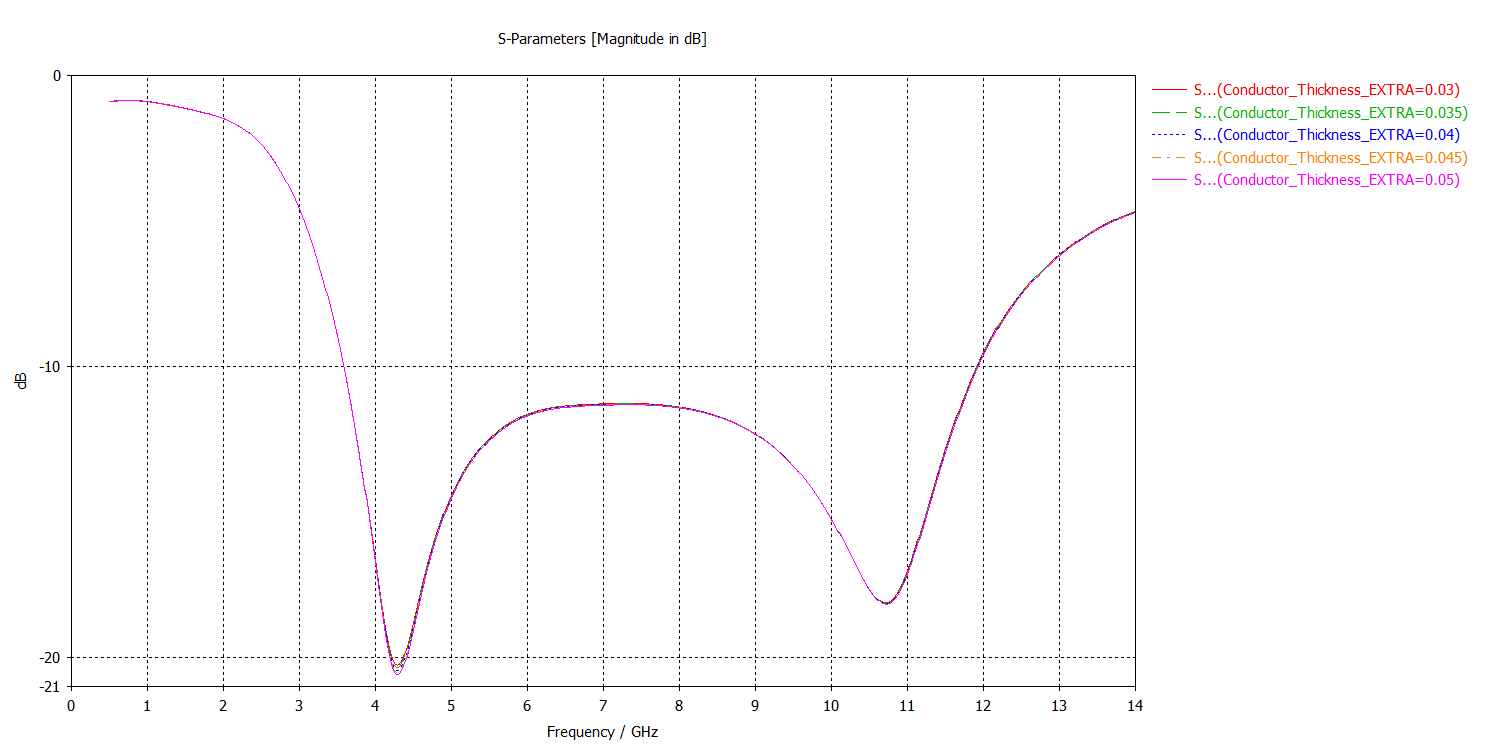
\includegraphics[width=14cm,valign=c]{Images/S1,1-conductor-thickness.png}\hspace{\fill}
	\caption{$S_{11}$ Parameters as material thickness is changed.}  %% Caption for your figure
	\label{fig:param_sweep_thickness}
\end{figure}

Other than what is listed above, I tried to follow the paper as closely as possible, even going as far as to alter CST's default value for the relative dielectric constant of FR-4 from 4.3 (CST's default) to 4.4 (what the paper lists as the dielectric constant for FR-4). \linebreak

\newpage




\subsection{Design and Simulation Set-up and Initial Results}
The first step I carried out for the design was to design the structure of the monopole device as per the paper and then set up the excitation port, and various field, current, etc. monitors for the antenna. I recreated all of the graphs (that can be recreated by CST) shown in the the original paper, these are labelled Figures 2 through 6 in the original document, you can see them below in Figure \ref{fig:paper_graph_recreation}: \linebreak


\begin{figure}[ht!]
\centering
	\begin{subfigure}[b]{0.45\linewidth}
    \centering
    	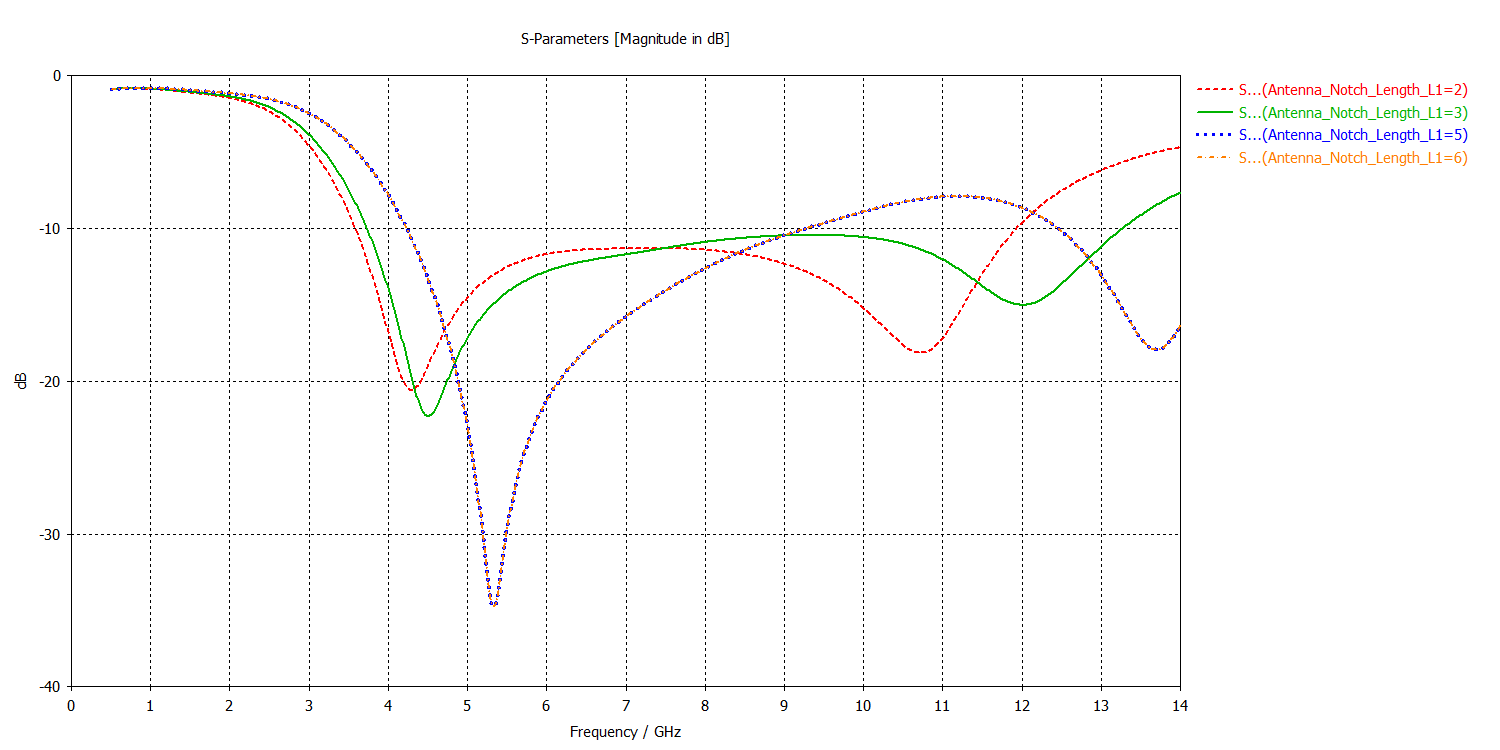
\includegraphics[width=0.95\textwidth]{Images/S1,1-fig-2-recreation.png}\\[2mm]
    	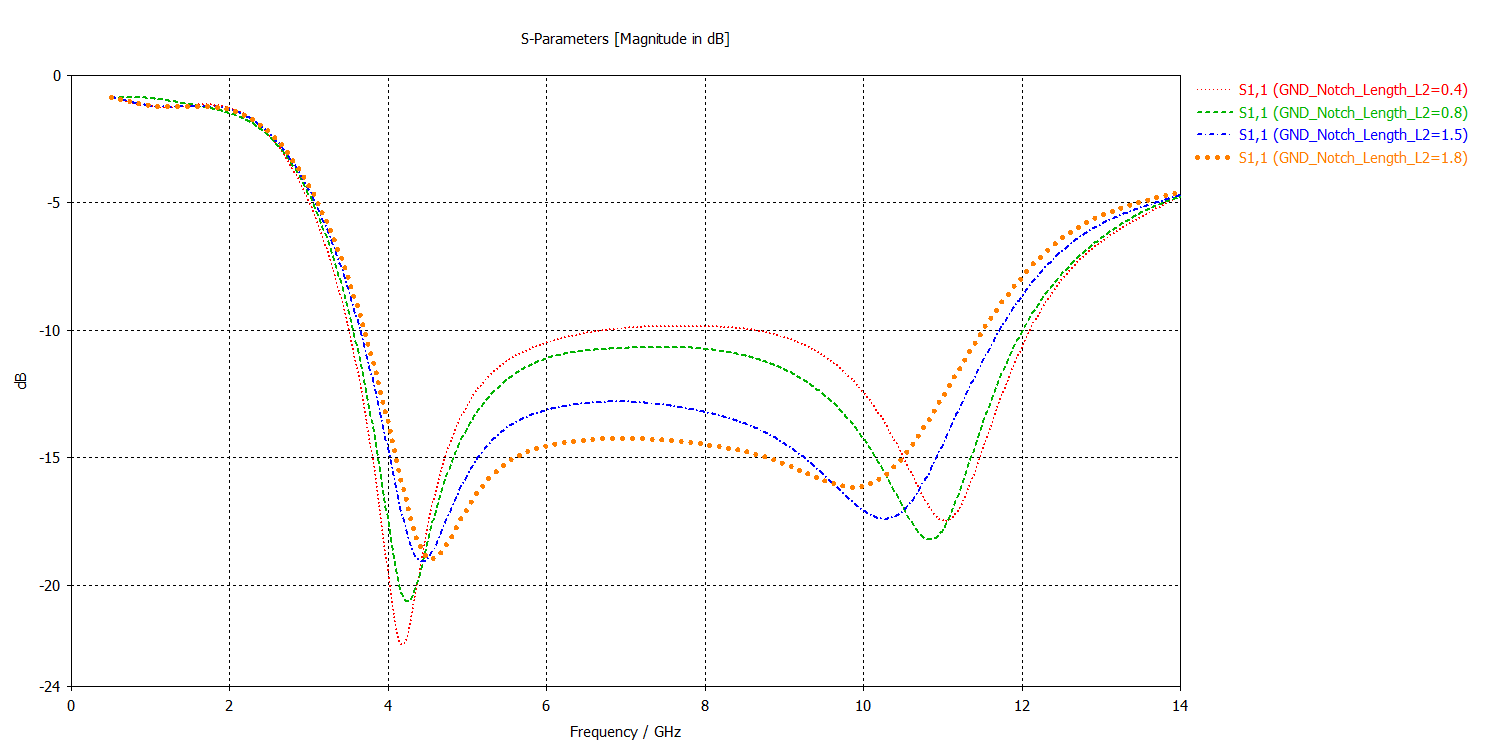
\includegraphics[width=0.95\textwidth]{Images/S1,1-fig-3-recreation.png}\\[2mm]
    	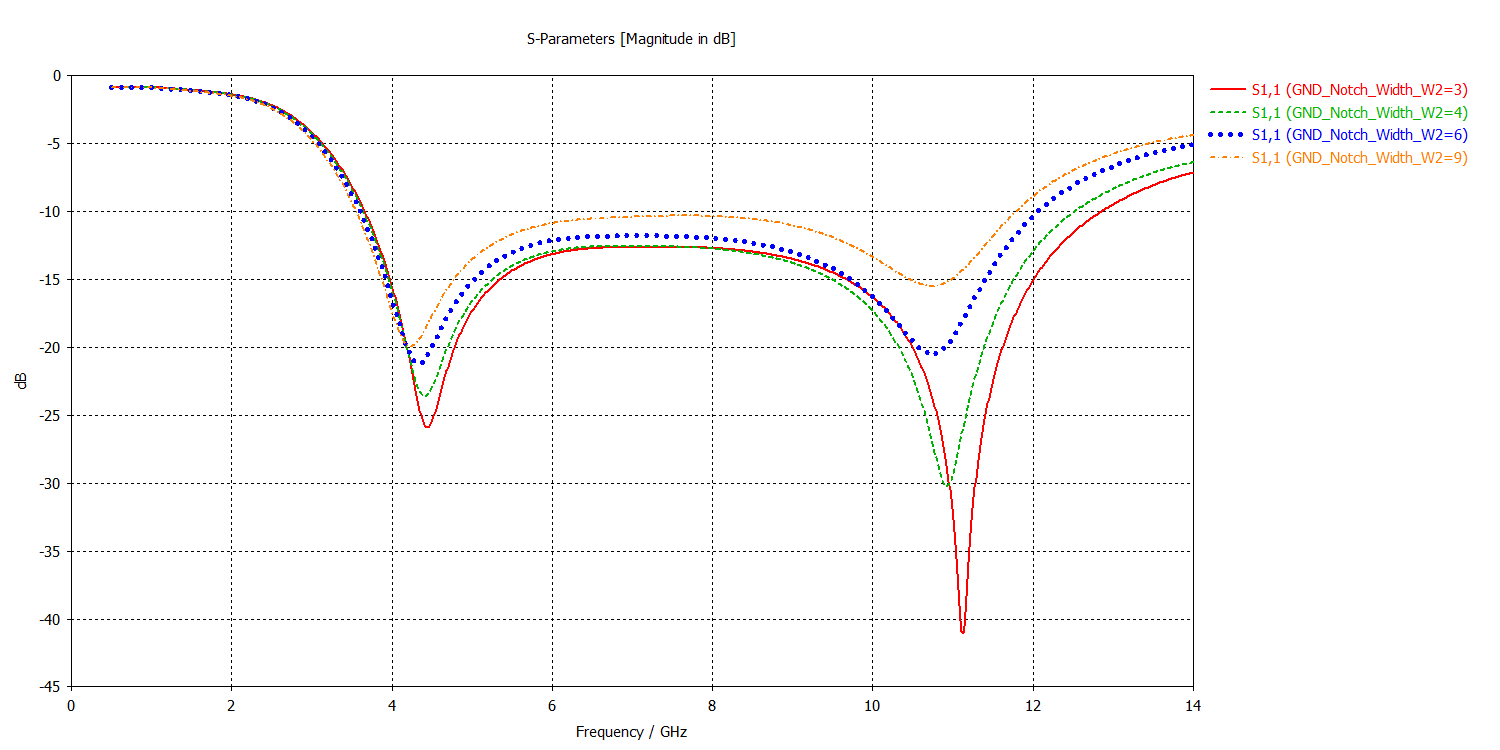
\includegraphics[width=0.95\textwidth]{Images/S1,1-fig-4-recreation.png}
    \caption{ Simulated return loss across a variation of lengths and widths, \\specifically the length of the two corner cut-outs of the monopole \\antenna ($L_1$), the truncated ground cut-out length ($L_2$), and \\truncated ground cut-out width ($W_2$), ordered top to bottom.}\label{fig:recreate_rtn_loss_param_sweeps}
	\end{subfigure}
	\begin{subfigure}[b]{0.45\linewidth}
	\centering
		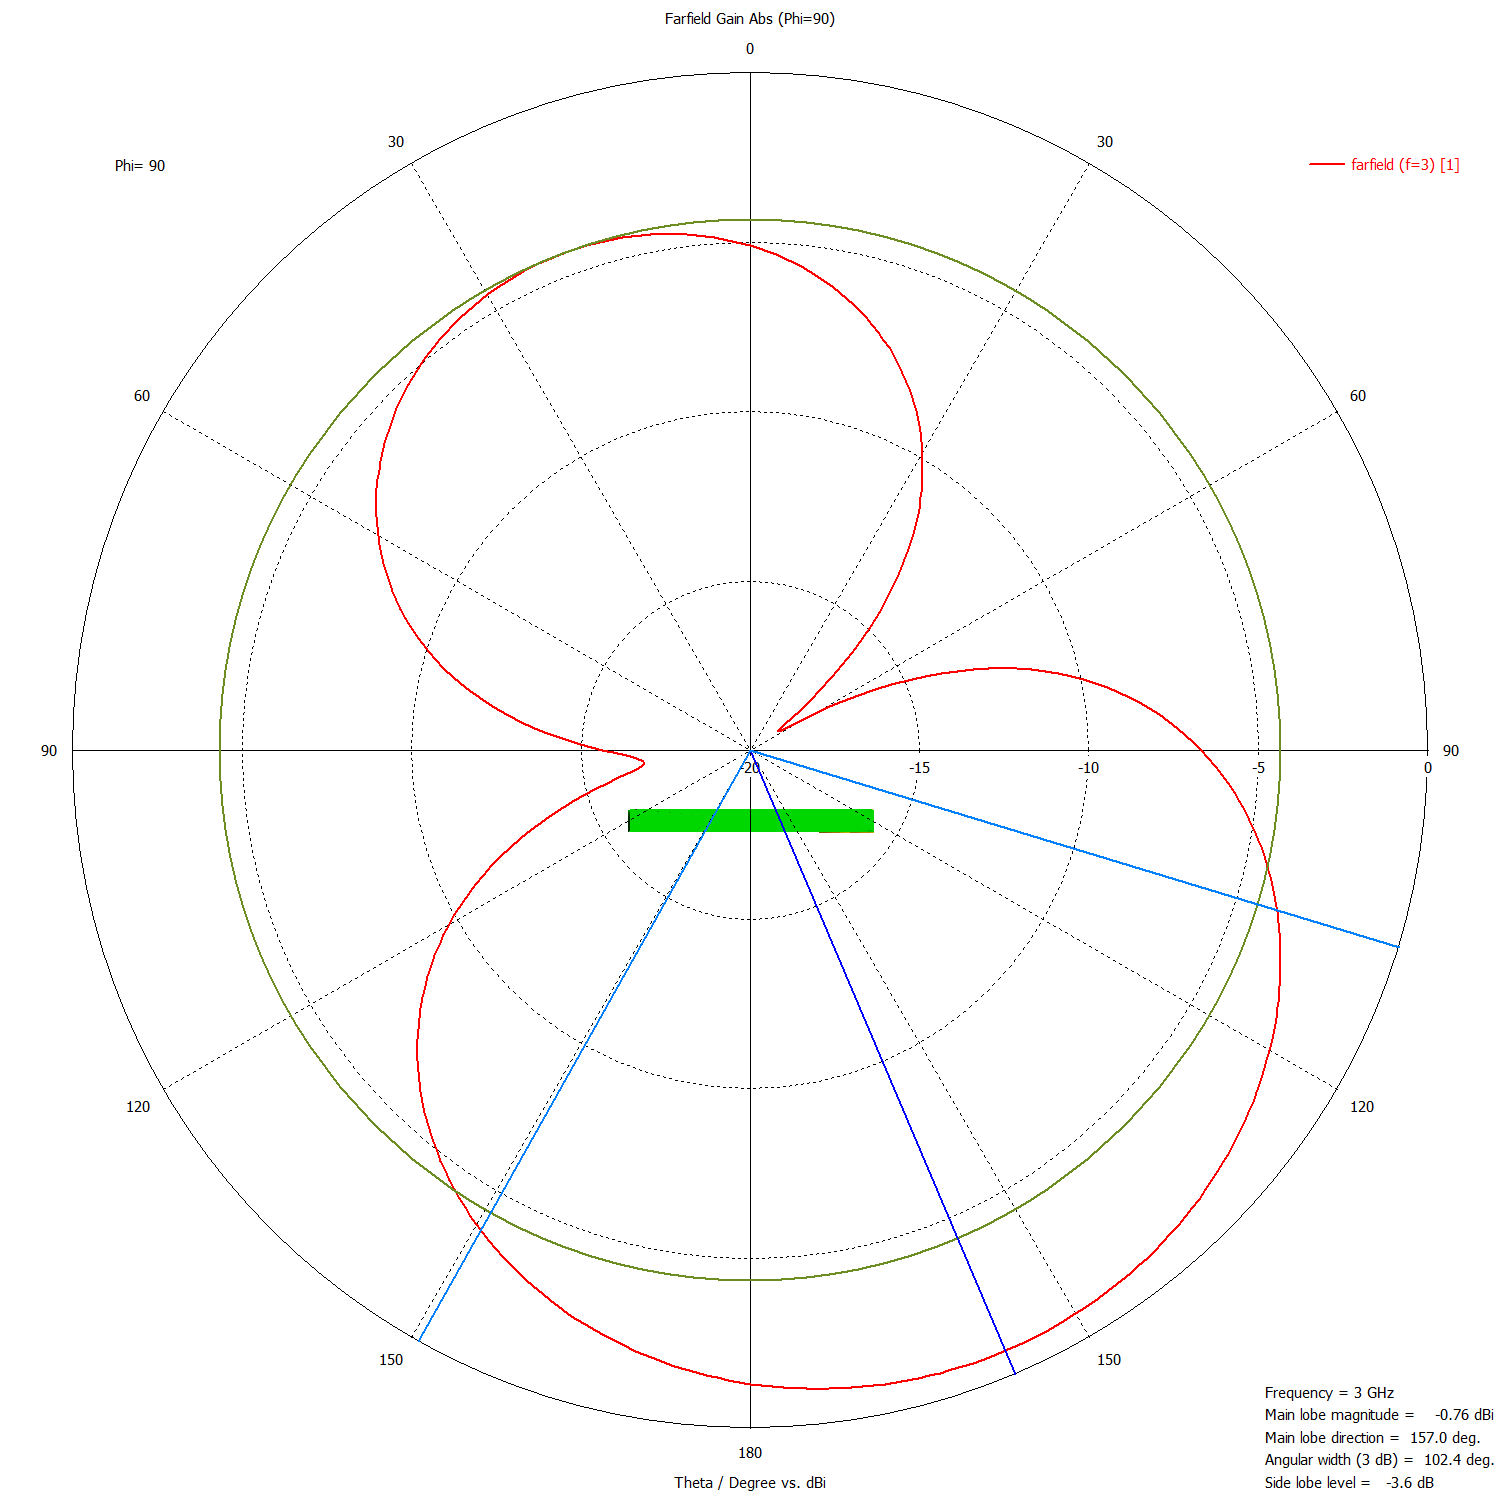
\includegraphics[width=0.45\textwidth]{Images/S1,1-fig-6-recreation-3GHz-YZ.png}
    	\hfill
		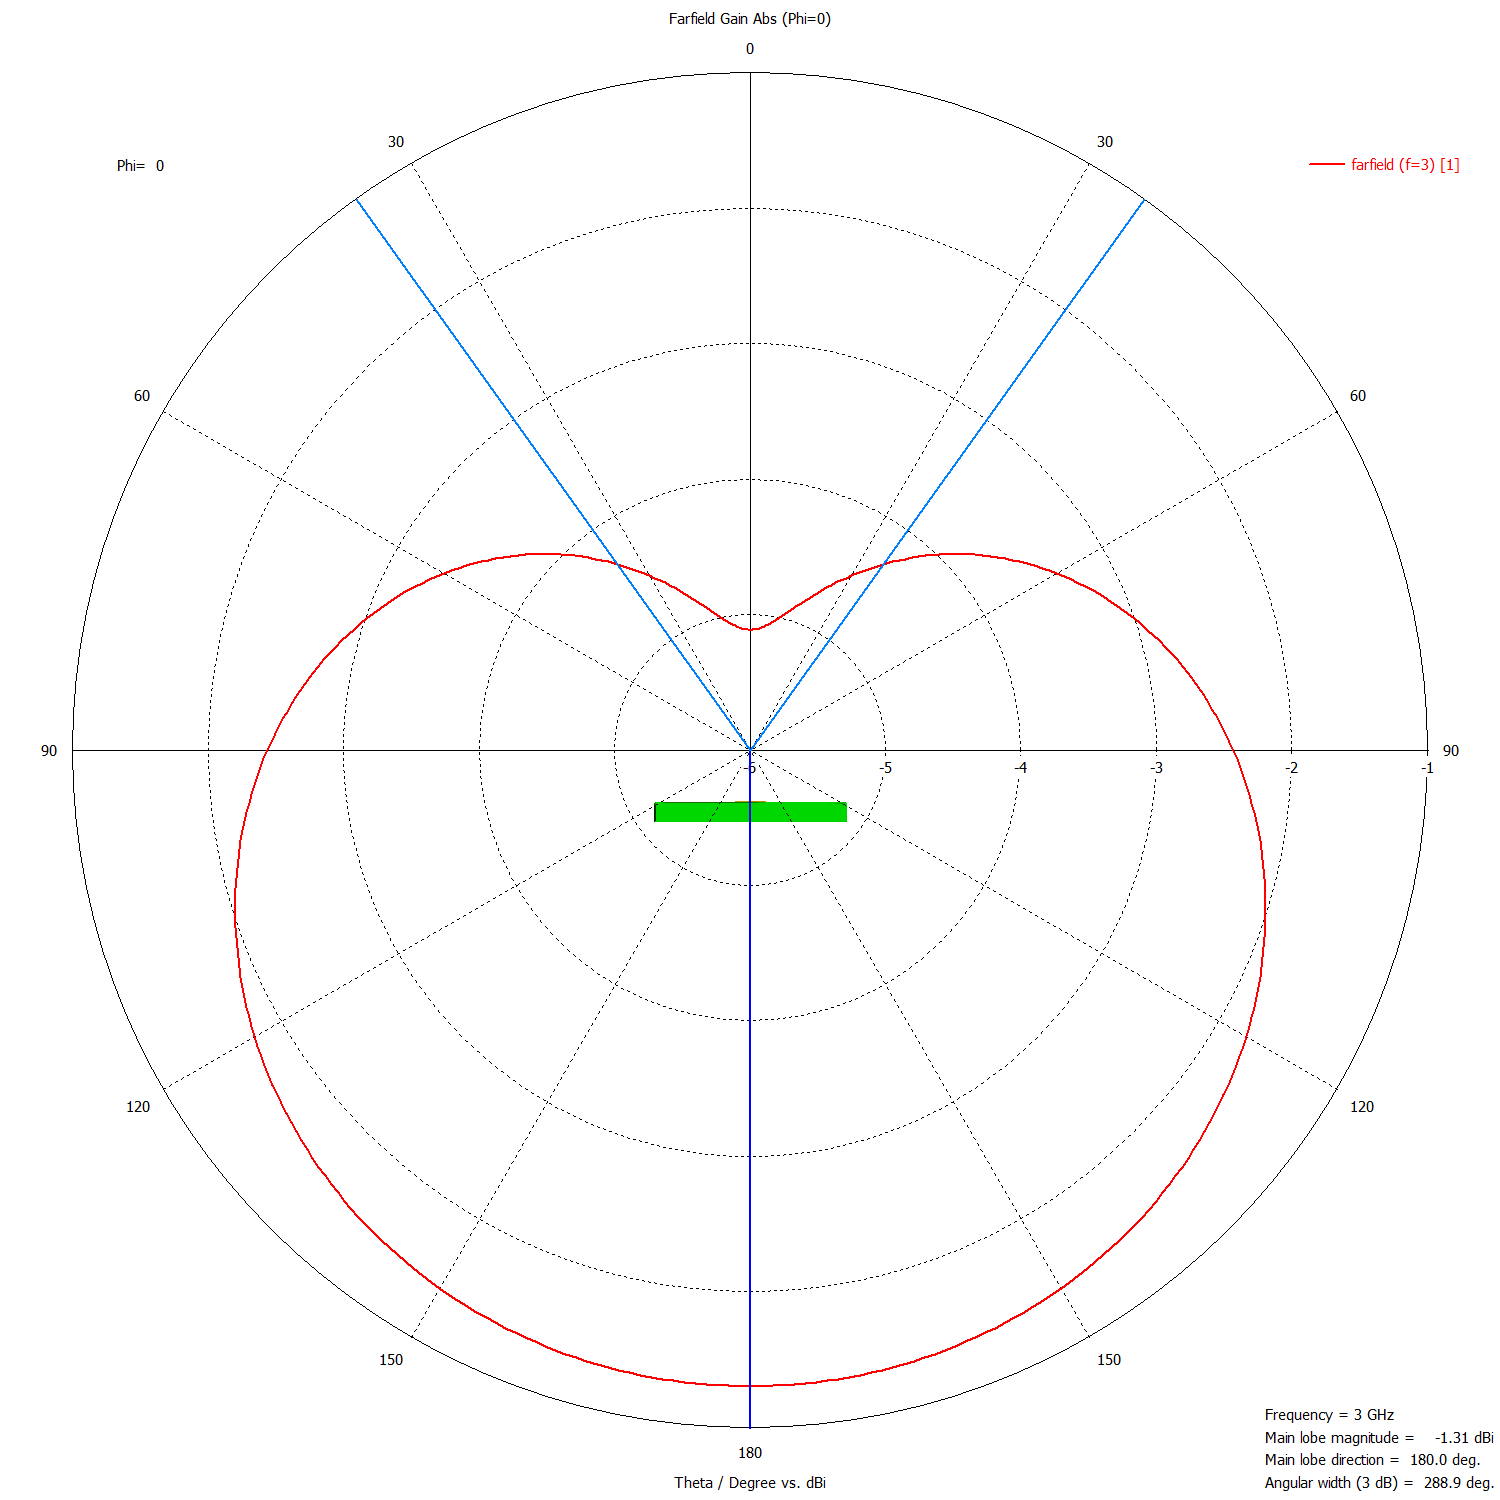
\includegraphics[width=0.45\textwidth]{Images/S1,1-fig-6-recreation-3GHz-XZ.png}\\[2mm]
		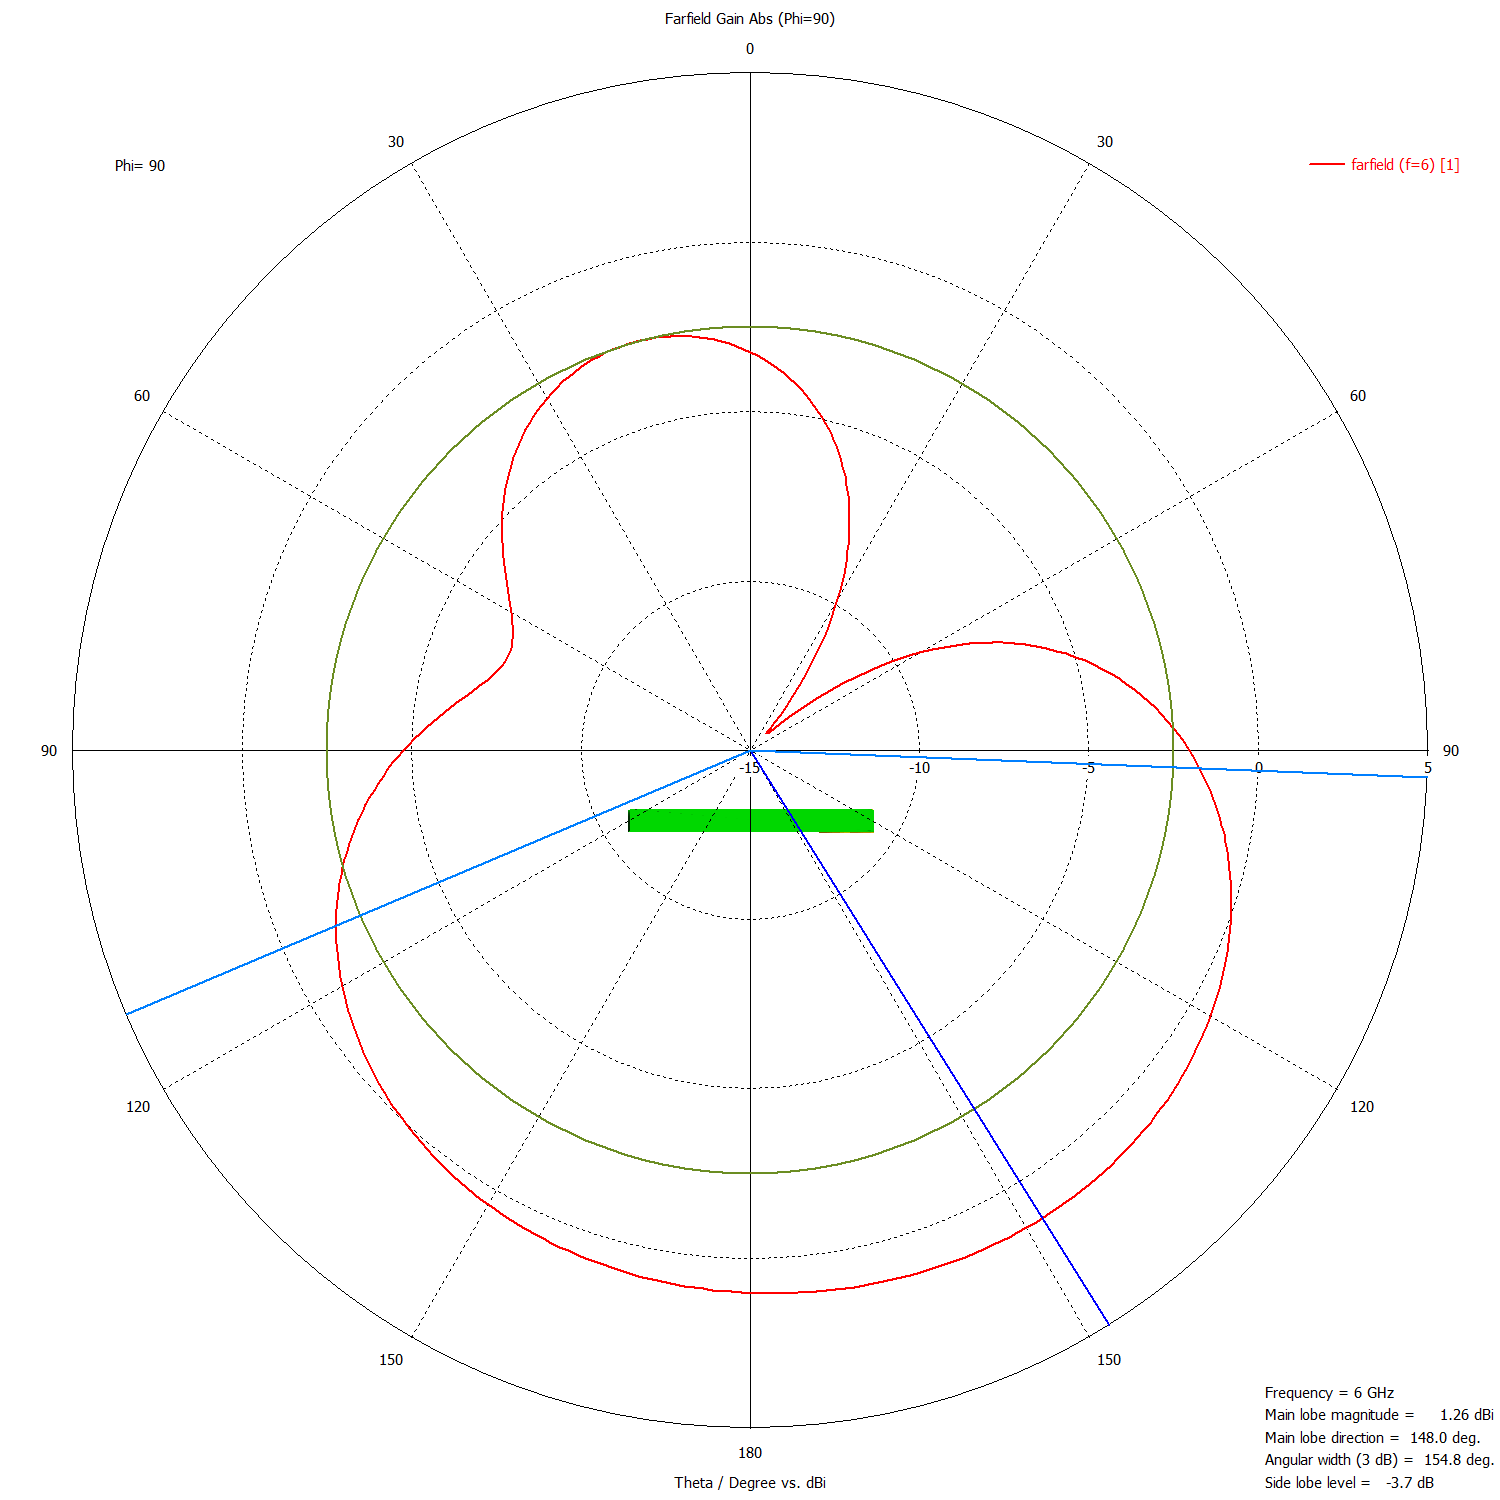
\includegraphics[width=0.45\textwidth]{Images/S1,1-fig-6-recreation-6GHz-YZ.png}
    	\hfill
		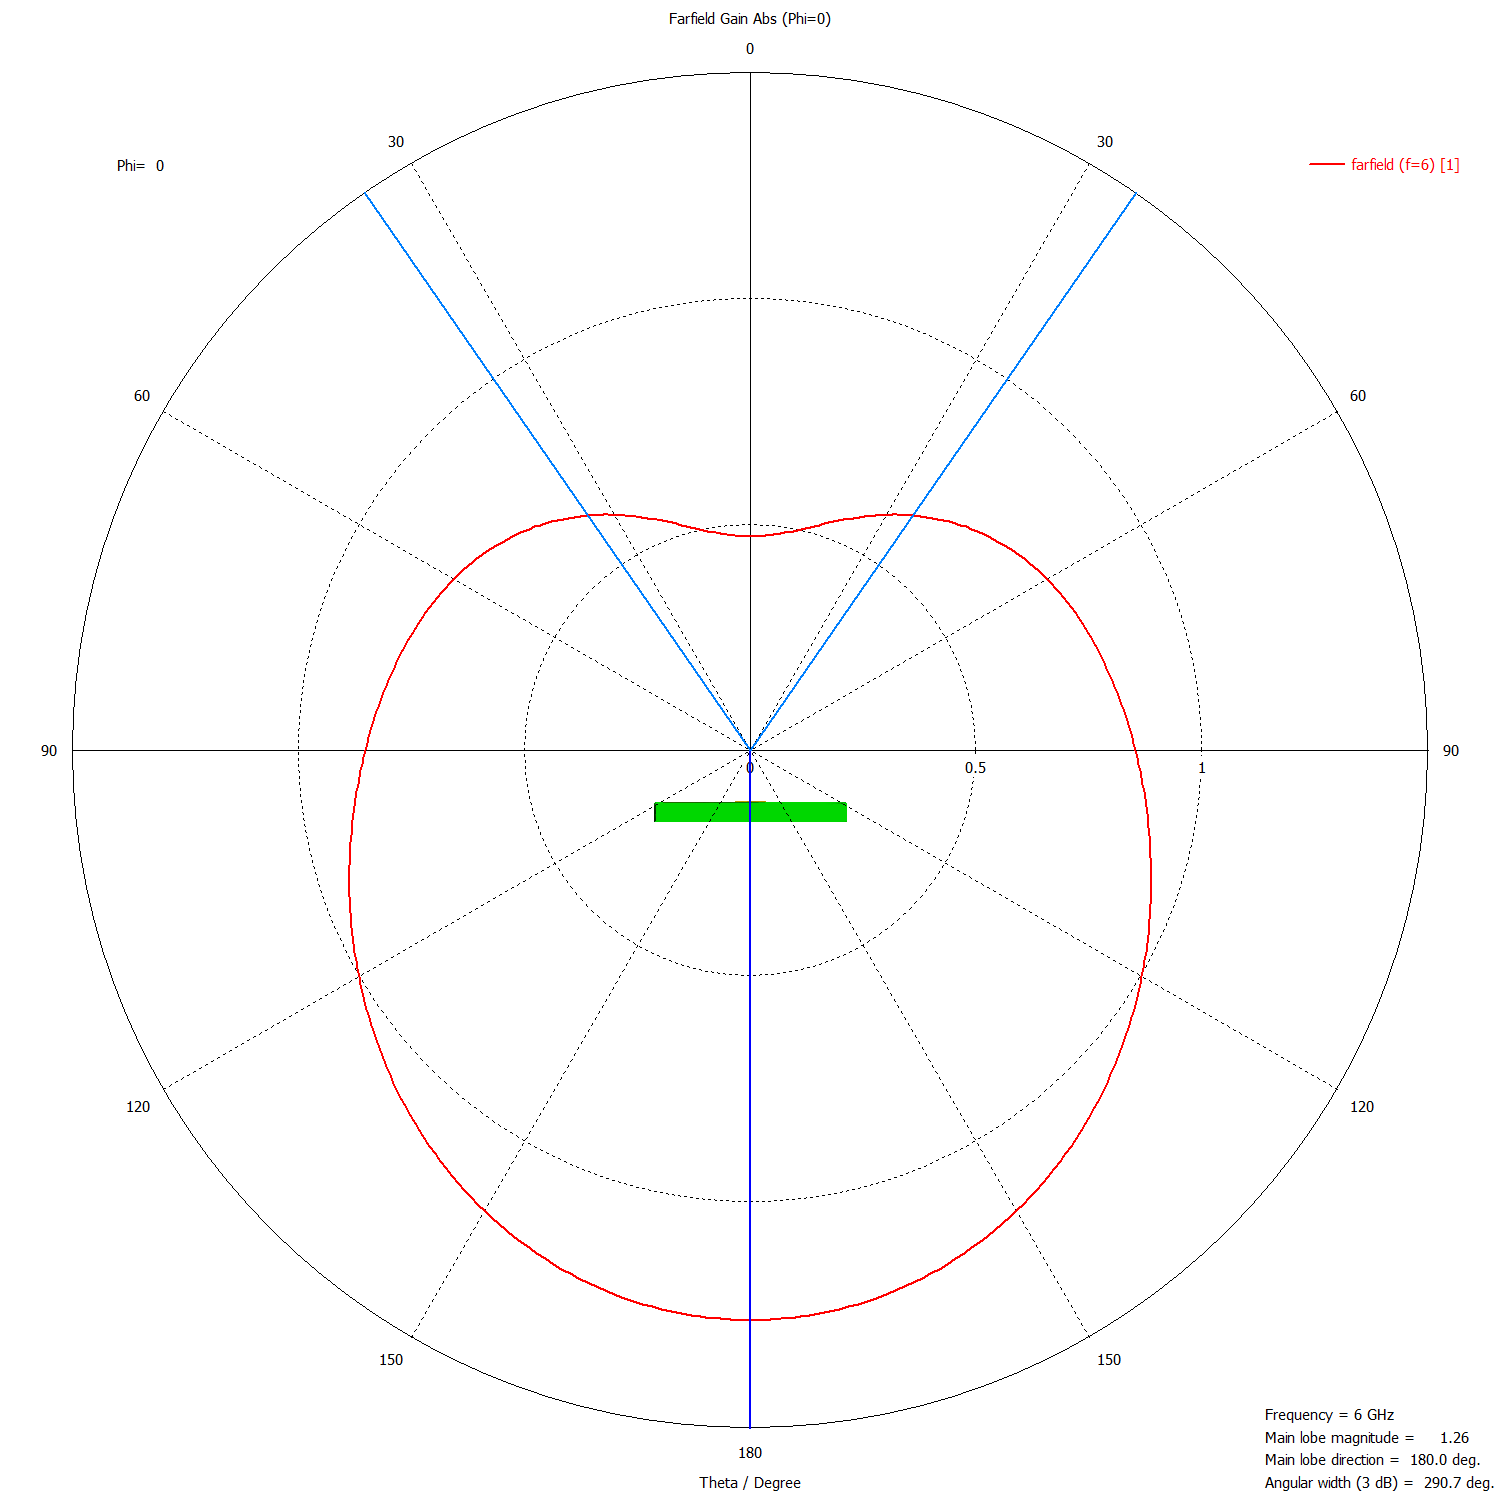
\includegraphics[width=0.45\textwidth]{Images/S1,1-fig-6-recreation-6GHz-XZ.png}\\[2mm]
		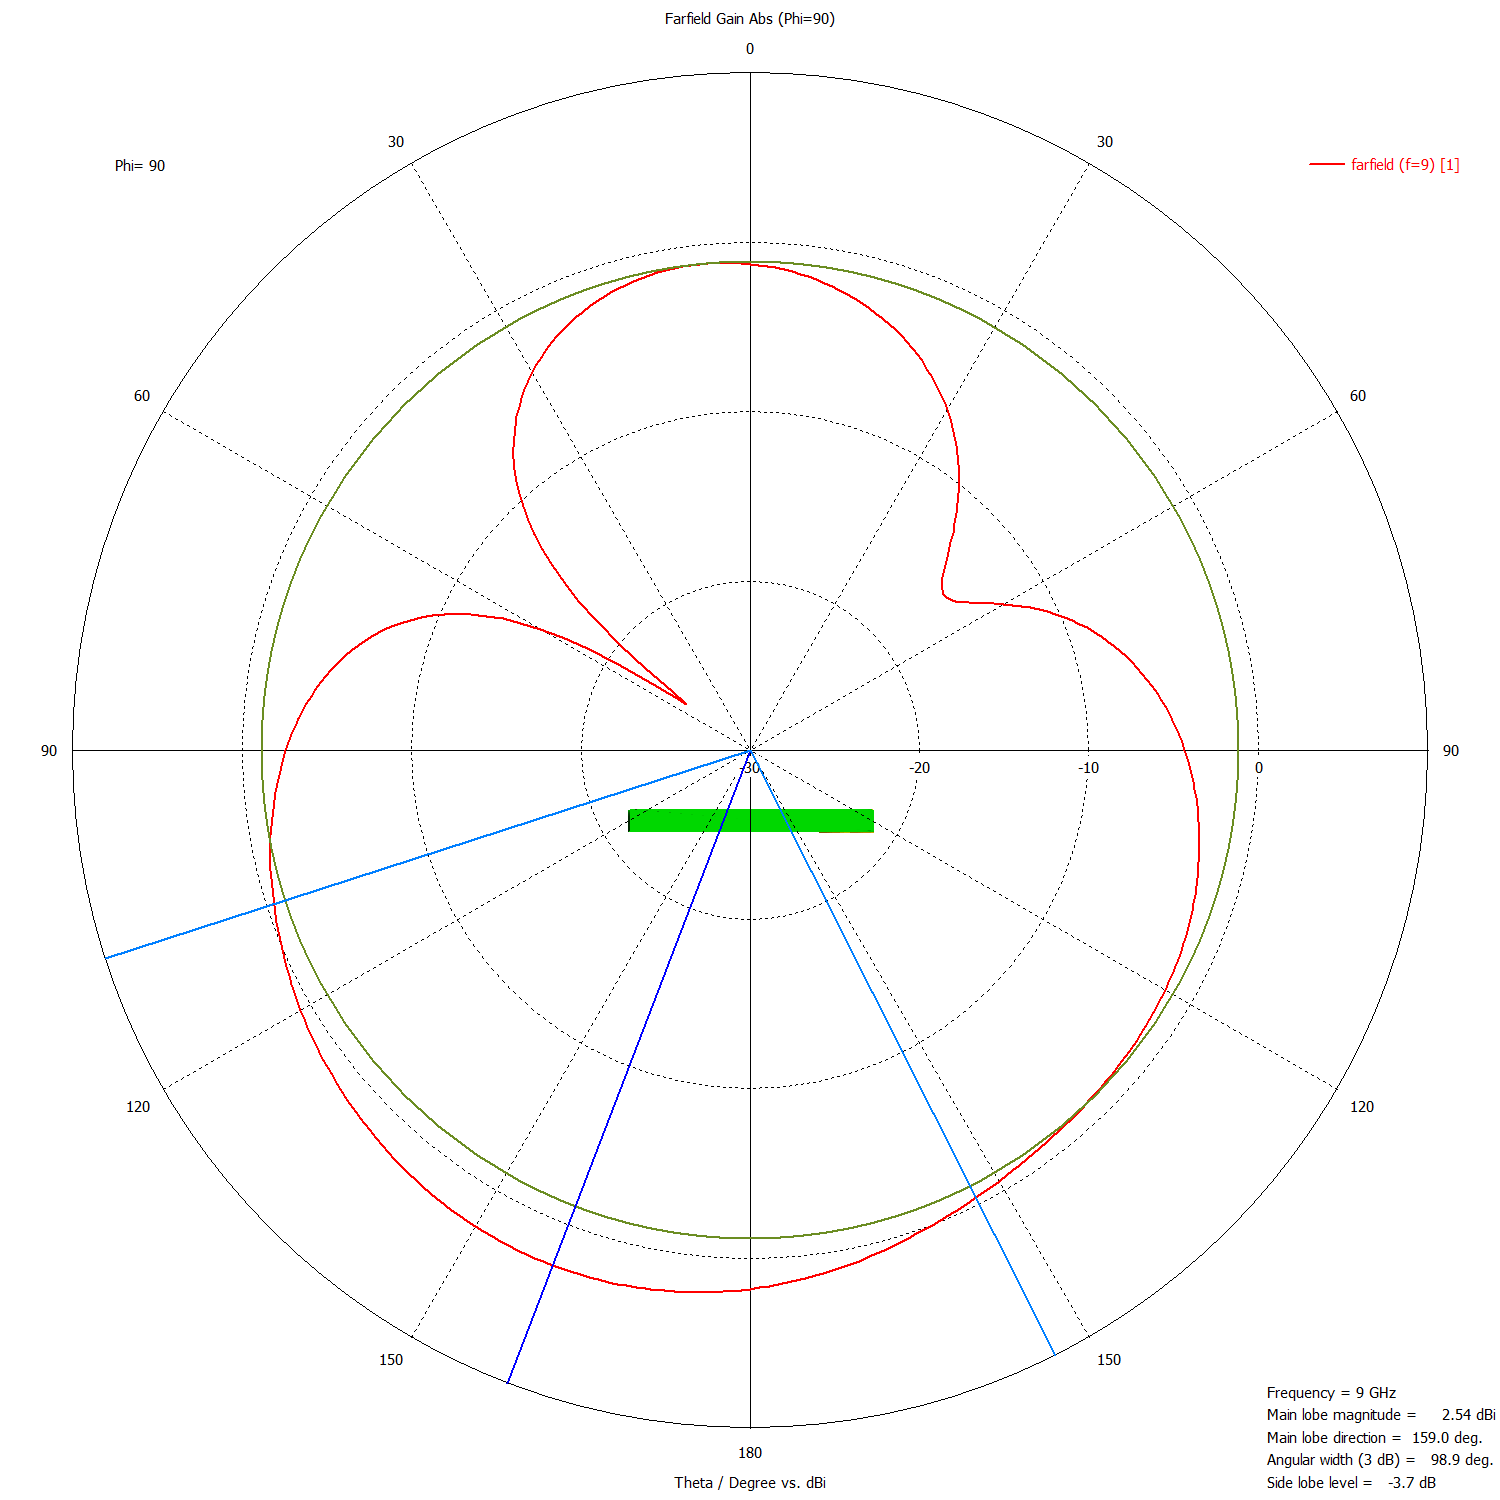
\includegraphics[width=0.45\textwidth]{Images/S1,1-fig-6-recreation-9GHz-YZ.png}
    	\hfill
		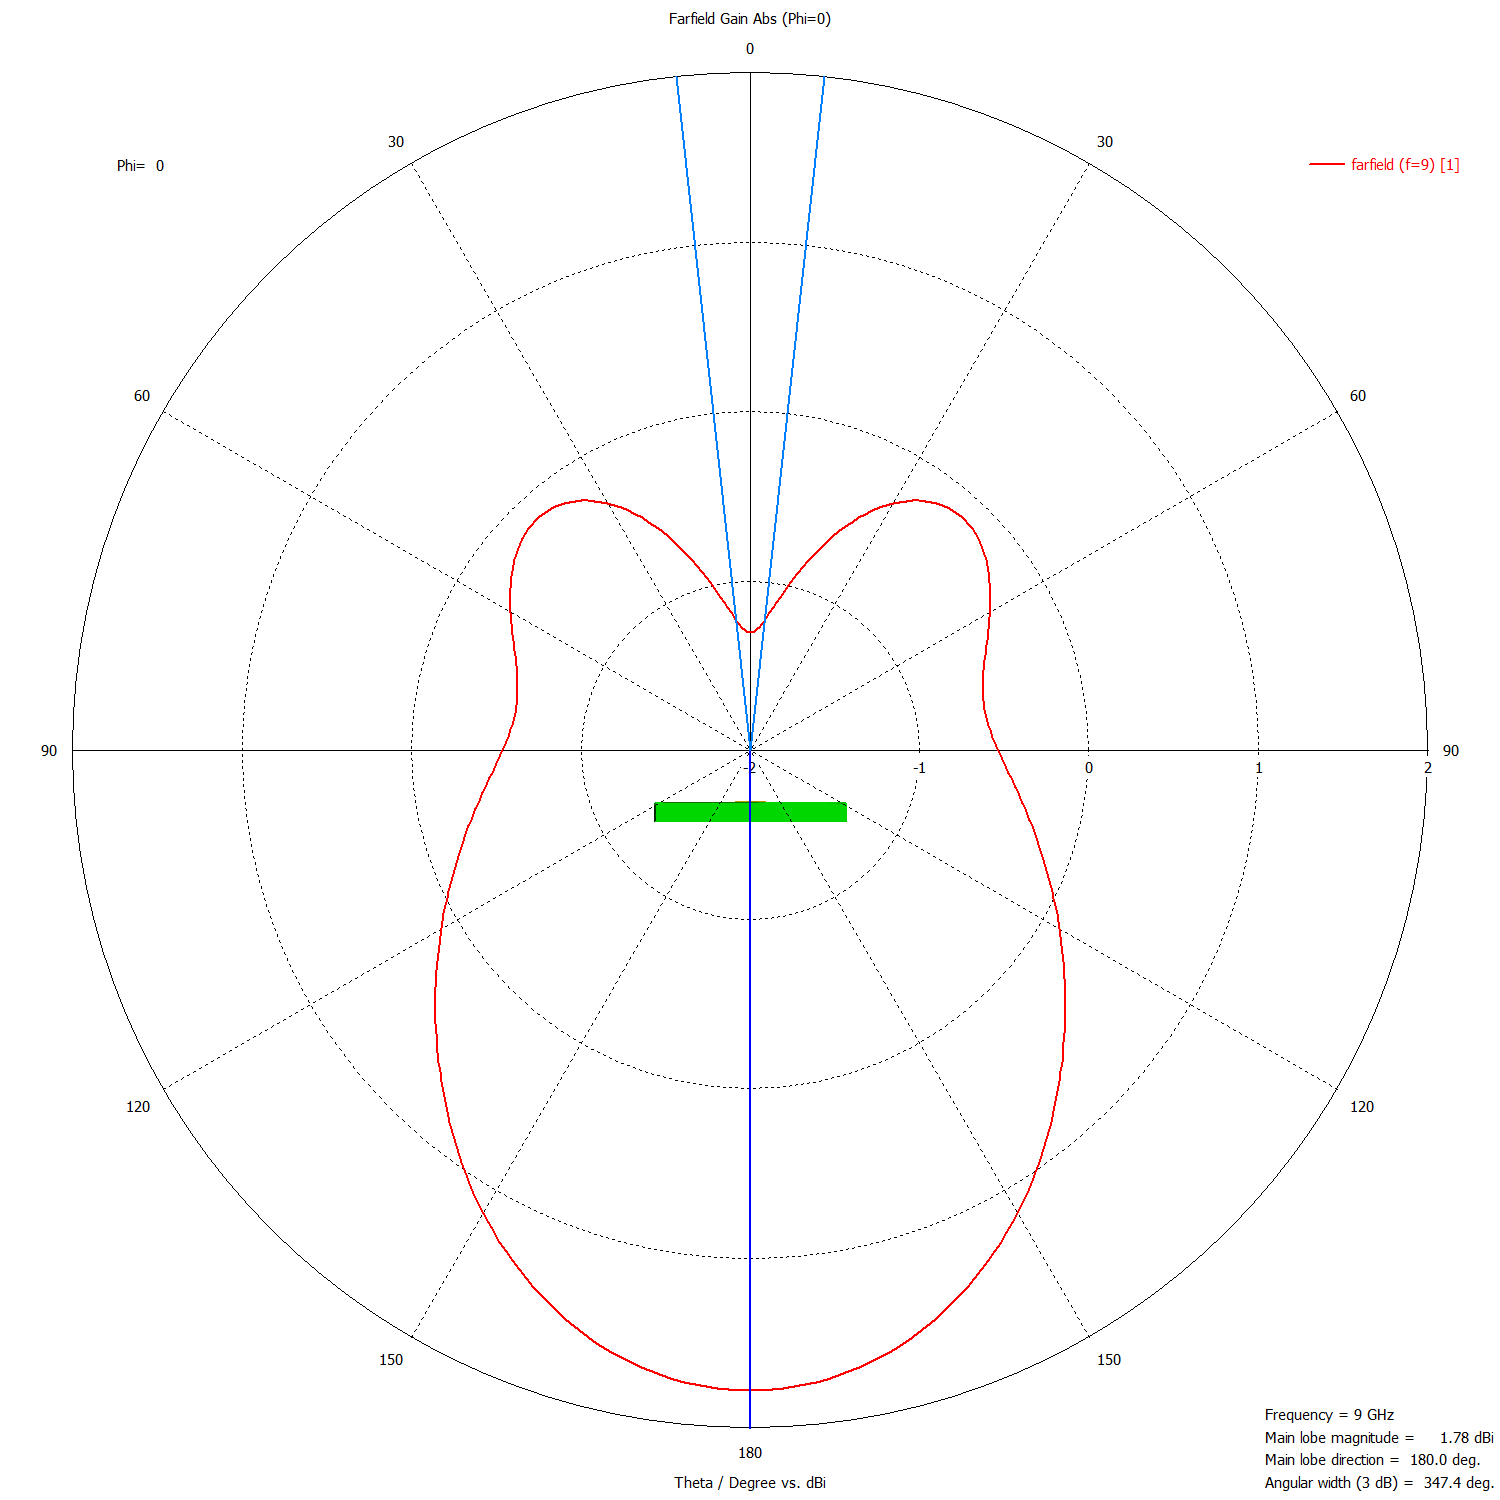
\includegraphics[width=0.45\textwidth]{Images/S1,1-fig-6-recreation-9GHz-XZ.png}
		\caption{Radiation patterns in the y-z and x-z plane (left and right respectively) at \\3 GHz, 6GHz, anf 9GHz (ordered top to bottom).}\label{fig:recreate_rad_patterns}
	\end{subfigure}
	\caption{A recreation of the graphs found in the paper.}\label{fig:paper_graph_recreation}
\end{figure}

\vspace{5mm}


The results obtained by CST when following the design specifications laid out in the paper are significantly different to that of the paper, so I strived to obtain a more accurate facsimile. I thought the most likely cause for the disparity could be that the port impedance was not actually 50$\mu$, so I ran a significant number of parameter sweeps on the width of the feeder micro-strip. The results from this simulation is shown below in Figure \ref{fig:microstrip_param_sweep}. \linebreak  
None of these results completely match that shown in the paper, and I ran many other simulations on a plethora of dimension parameters in an attempt to recreate the results of the paper, however there is not enough room in this report to present all of those attempts. In the next Section I present the results of my selected optimised values. \linebreak


\begin{figure}[ht]
	\centering
	\hspace{\fill}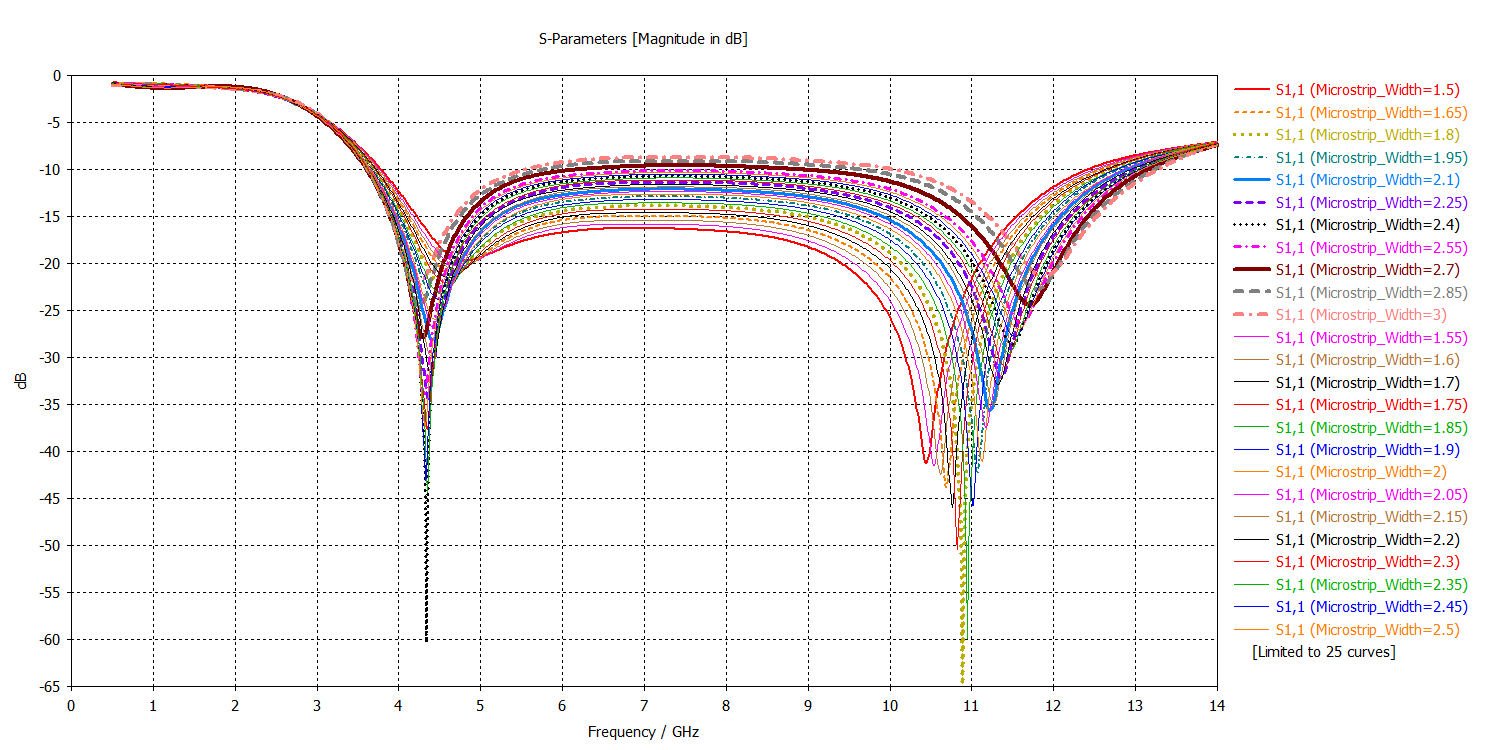
\includegraphics[width=14cm,valign=c]{Images/S1,1-microstrip-param-sweep.png}\hspace{\fill}
	\caption{$S_{11}$ Parameters as the feeding micro-strip width is changed.}  %% Caption for your figure
	\label{fig:microstrip_param_sweep}
\end{figure}


\newpage




\section{Final Results and Discussion}
The final results are obtained from a set of dimensions I chose in order to try to strike a balance between minimal average return loss and as wide an operating bandwidth as possible. The final dimensions I chose are: $W_2=3mm$ and Microstrip Width = 1.9mm, compared to $W_2=7mm$ and Microstrip Width = 2mm used in the paper. The resulting return loss graph from my chosen dimensions is shown below in Figure \ref{fig:s11_optimised}. These display a good bandwidth (~3.7Ghz to ~12.5GHz) and a very good average return loss across the bandwidth, there is enough of a tolerance that a manufactured version of the antenna should be able to realistically operate across the bandwidth. \linebreak
These results, again, obviously do not perfectly replicate the paper but are close enough and are a result from enough simulation on part to make it as close as possible to the paper. \linebreak 


\begin{figure}[ht]
	\centering
	\hspace{\fill}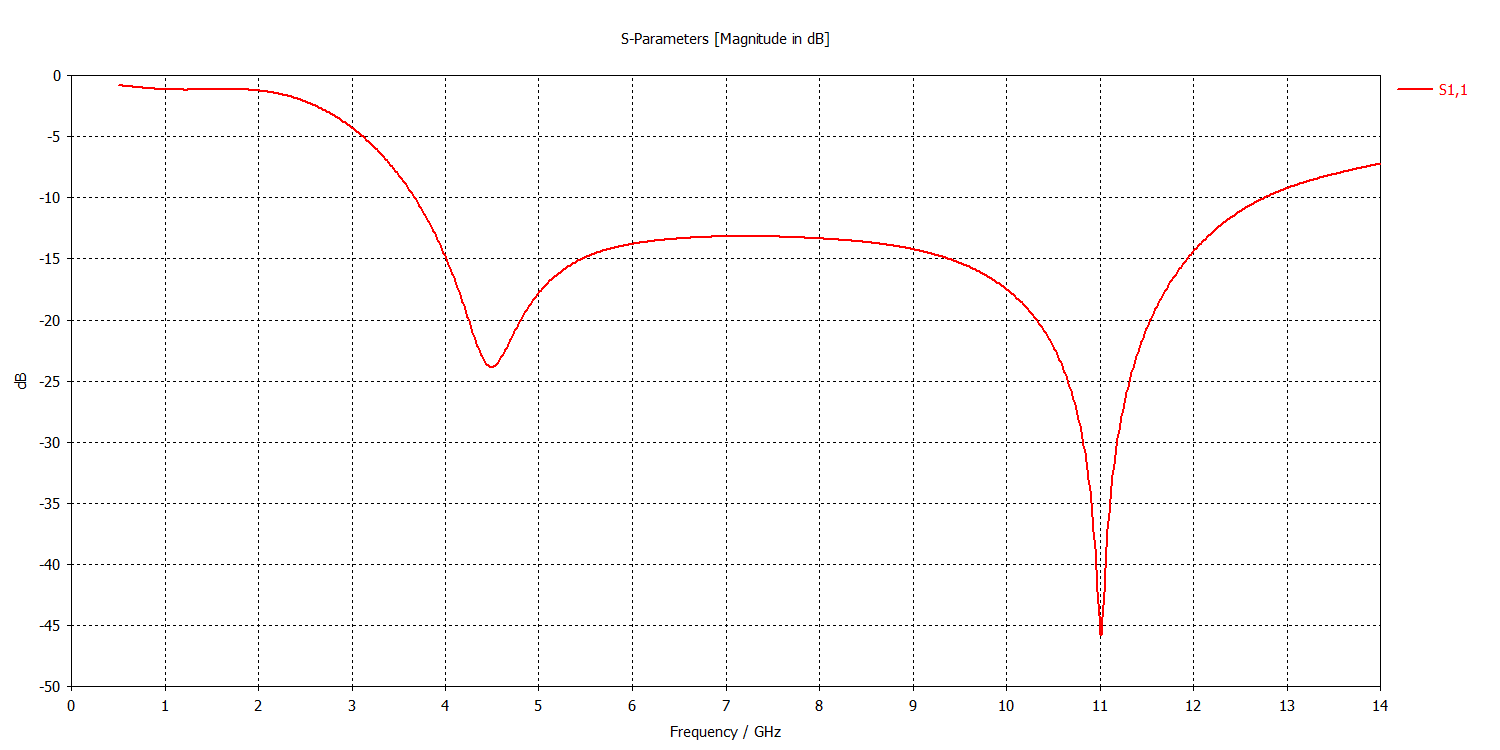
\includegraphics[width=14cm,valign=c]{Images/S1,1-optimised-values.png}\hspace{\fill}
	\caption{$S_{11}$ Parameters of the optimised antenna}  %% Caption for your figure
	\label{fig:s11_optimised}
\end{figure}


\newpage


Looking at the current density distribution of the antenna at it's resonant frequencies, and it's central frequency (4.5GHz, 11GHz, and 7.5GHz respectively) shows that the current at the resonant frequencies and across the bandwidth is concentrated through the micro-strip after which it dissipates, which is to be expected considering that it should be radiating out from the rest of the antenna. A 3D representation of the current density is shown in Figure \ref{fig:current_densities}. \linebreak

\begin{figure}[ht!]
\centering

		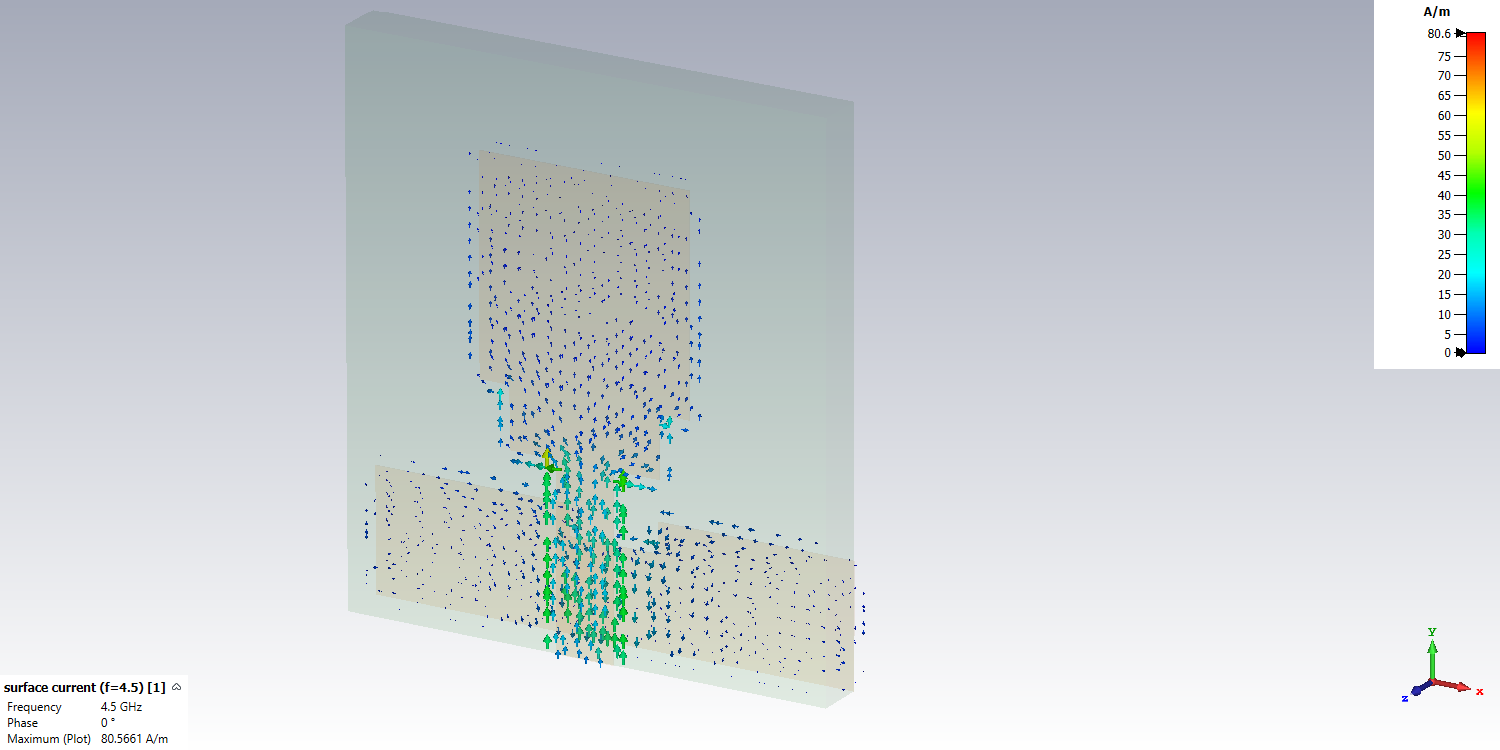
\includegraphics[width=0.3\textwidth]{Images/current-density-4.5GHz.png}
    	\hfill
		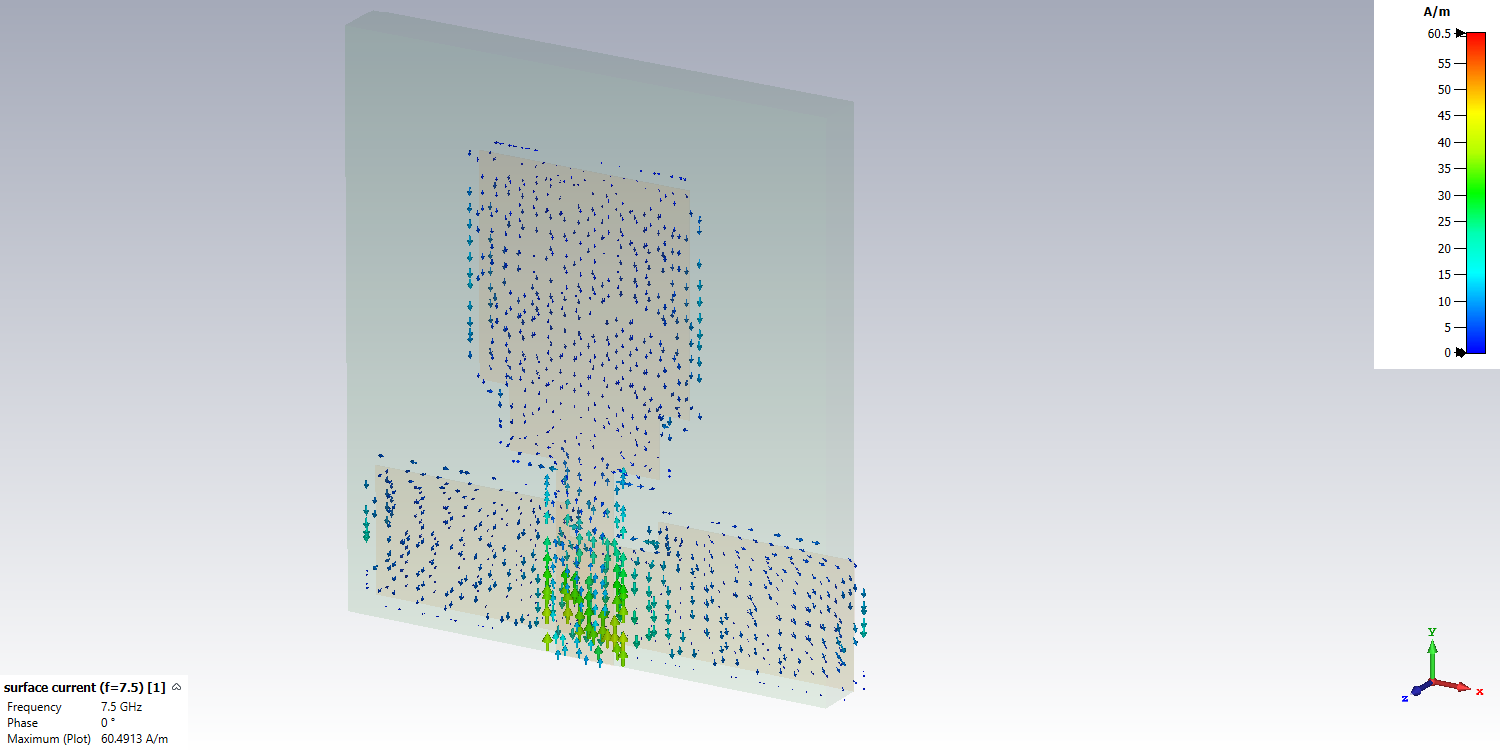
\includegraphics[width=0.3\textwidth]{Images/current-density-7.5GHz.png}
		\hfill
		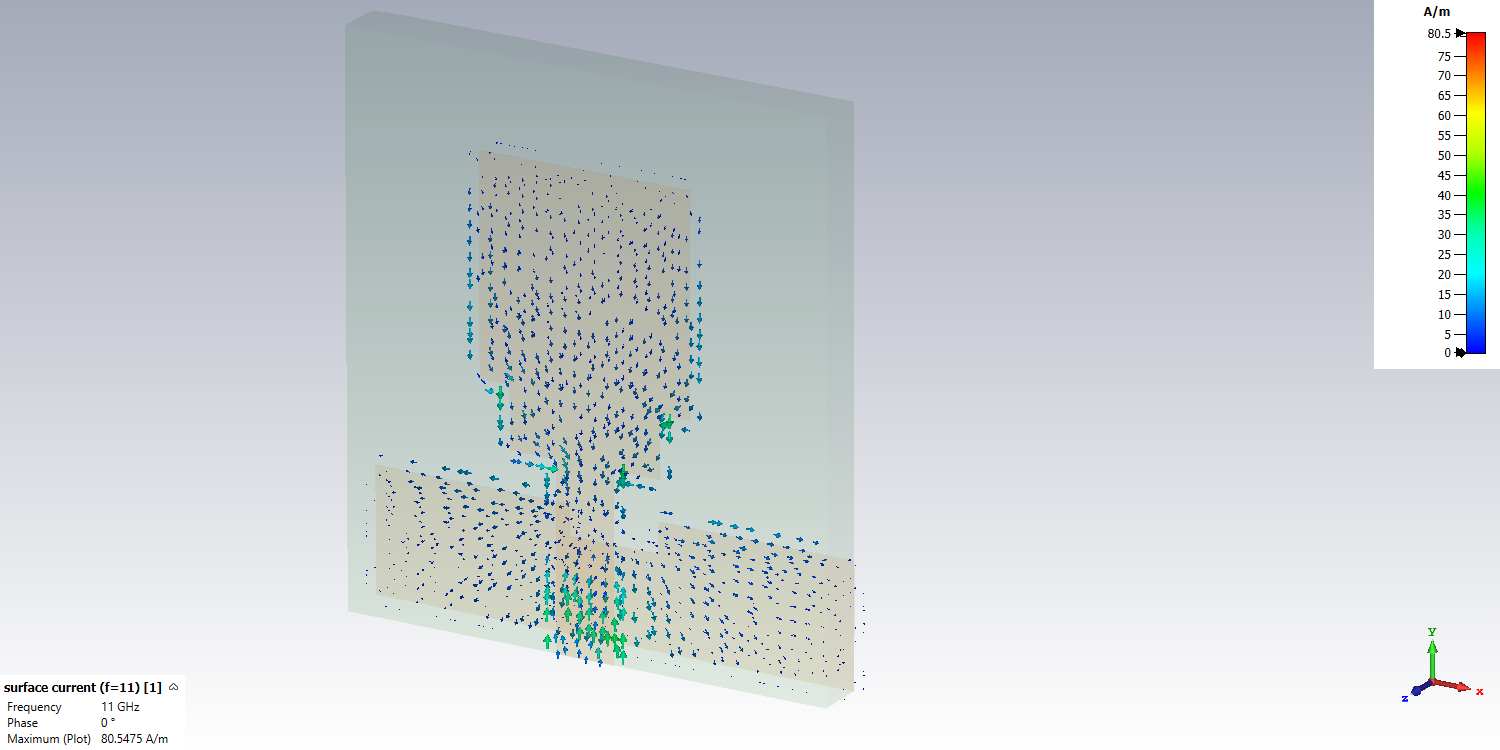
\includegraphics[width=0.3\textwidth]{Images/current-density-11GHz.png}
	\caption{3D images of the current density at 4.5GHz, 7.5GHz, \& 11GHz}\label{fig:current_densities}
\end{figure}

\vspace{5mm}

The magnetic and electric fields of the antenna at it's resonant frequencies, and it's central frequency (4.5GHz, 11GHz, and 7.5GHz respectively) also show an expected story, the magnetic field circles around the antenna's y-axis and the electric field is flowing towards the ground plane in a fashion very similar to that of a micro-strip transmission line. The fields also help to explain the far-field results shown later, the far-field is heavily directional, concentrating towards the ground plane with low gain in a lot of other directions. Figures \ref{fig:mag_field} and \ref{fig:electric_field} display the magnetic and electric fields respectively. \linebreak

\begin{figure}[ht!]
\centering

		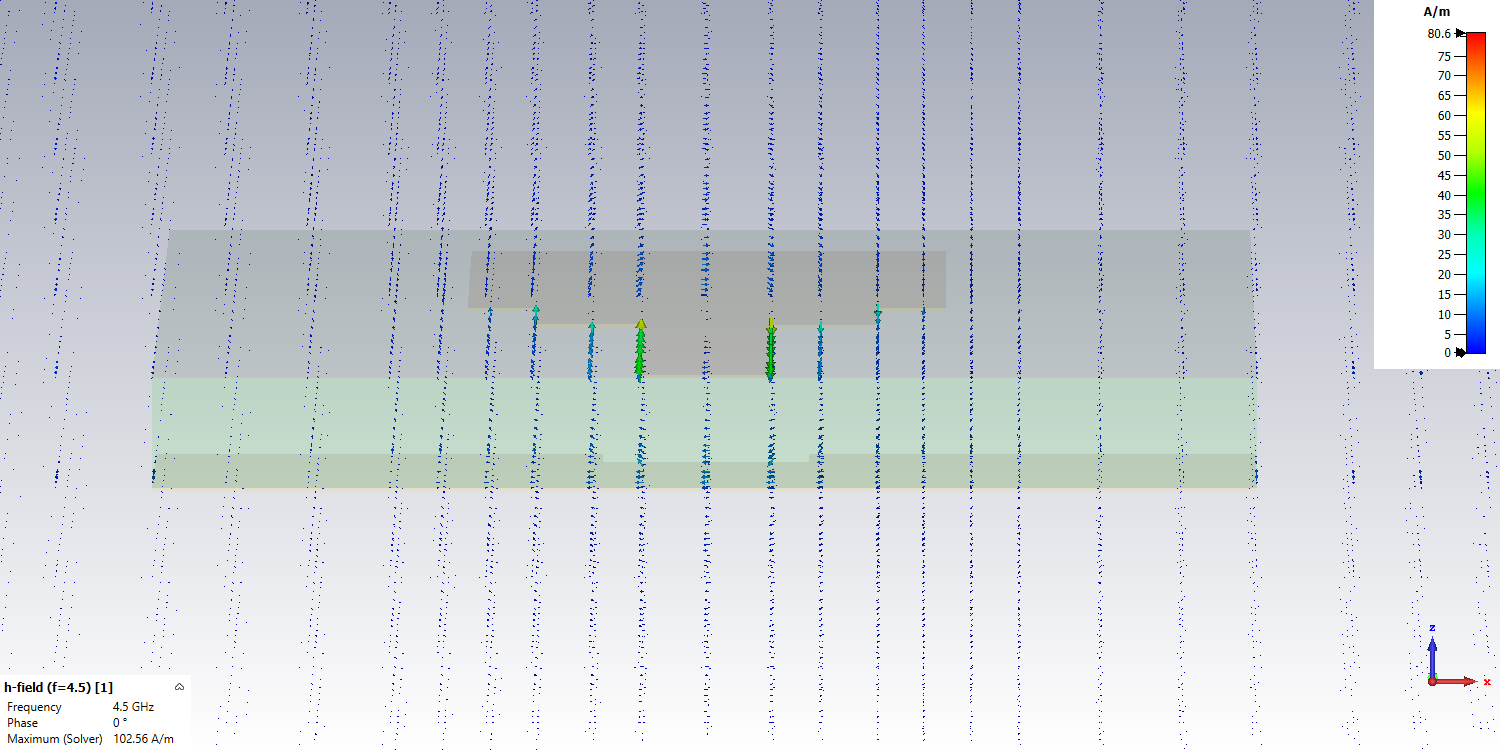
\includegraphics[width=0.3\textwidth]{Images/mag-field-4.5GHz.png}
    	\hfill
		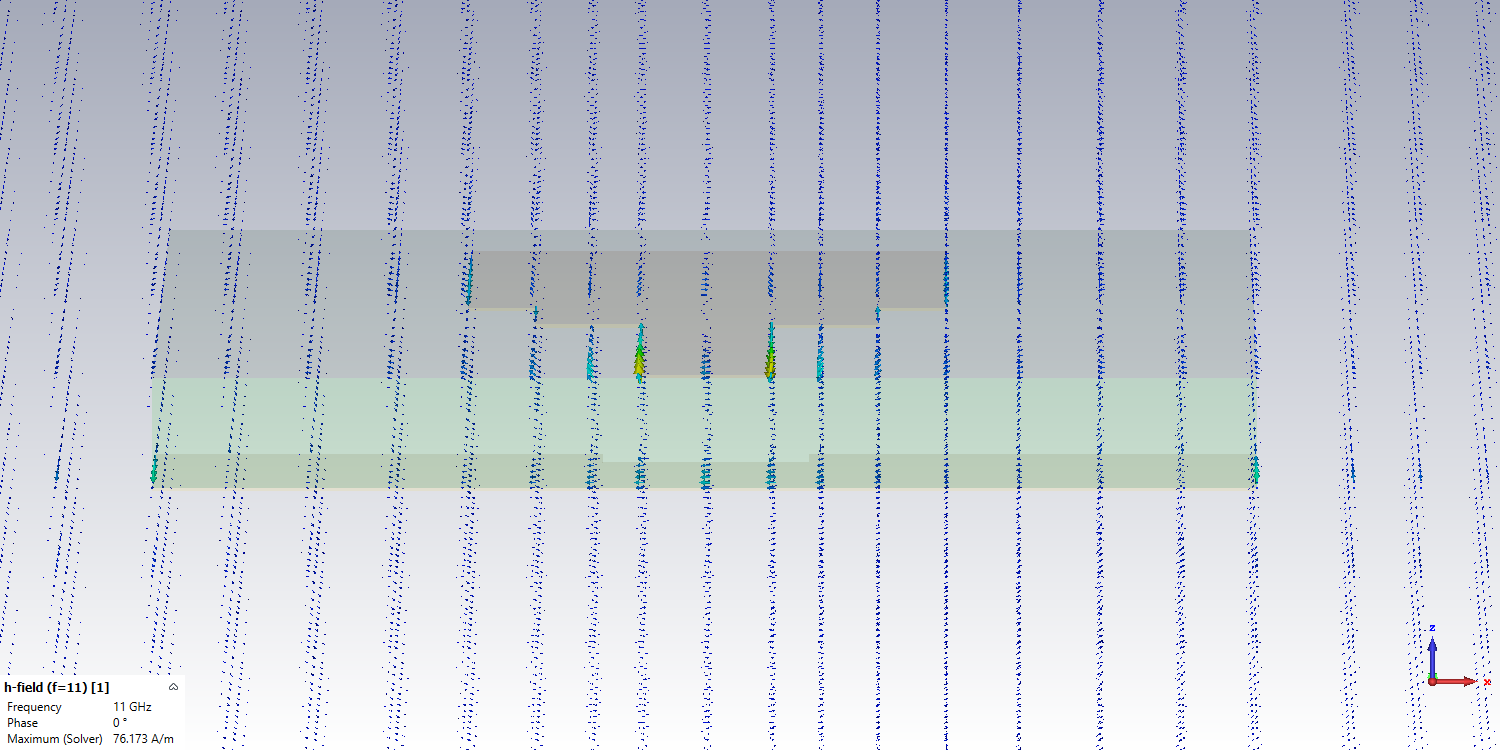
\includegraphics[width=0.3\textwidth]{Images/mag-field-7.5GHz.png}
		\hfill
		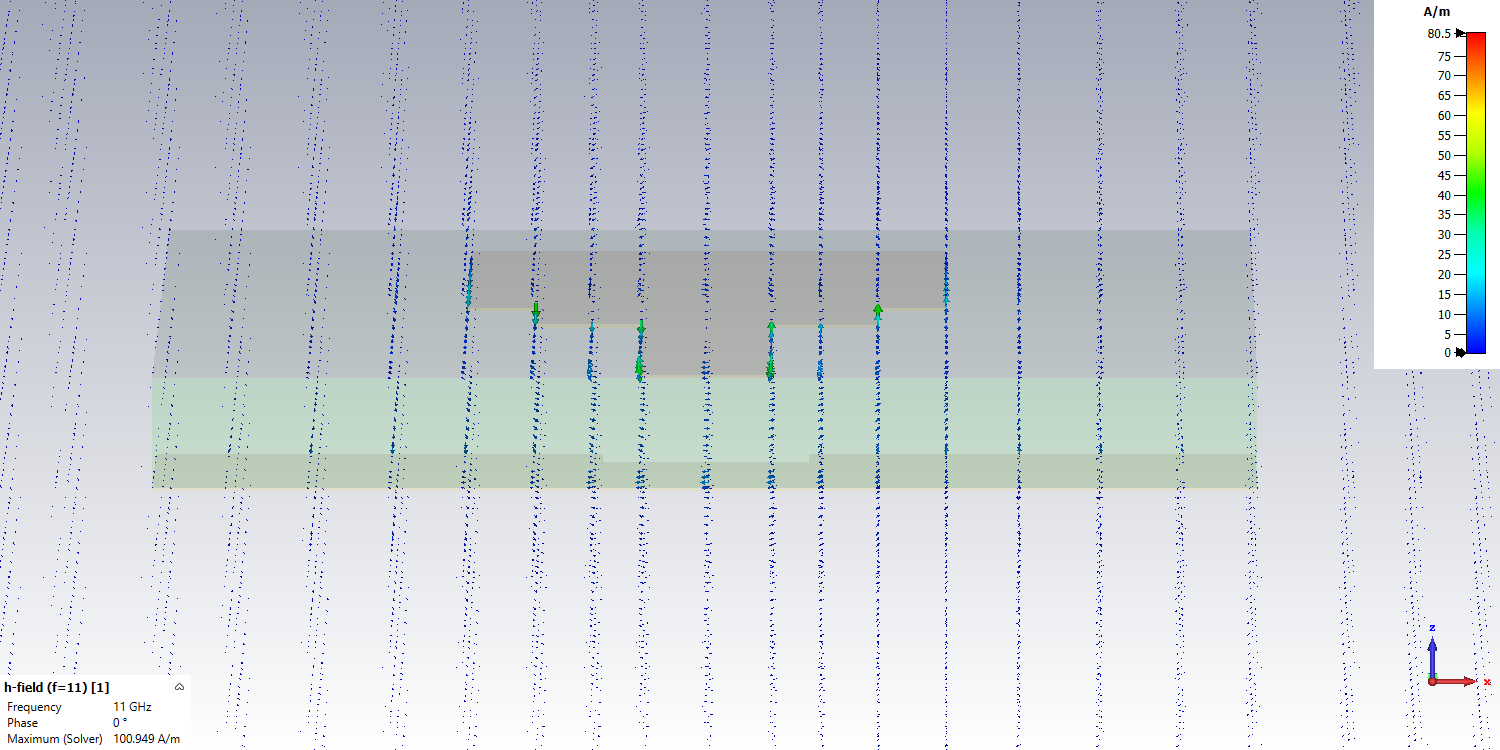
\includegraphics[width=0.3\textwidth]{Images/mag-field-11GHz.png}
	\caption{3D images of the magnetic field at 4.5GHz, 7.5GHz, \& 11GHz}\label{fig:mag_field}
\end{figure}

\vspace{5mm}

\begin{figure}[ht!]
\centering

		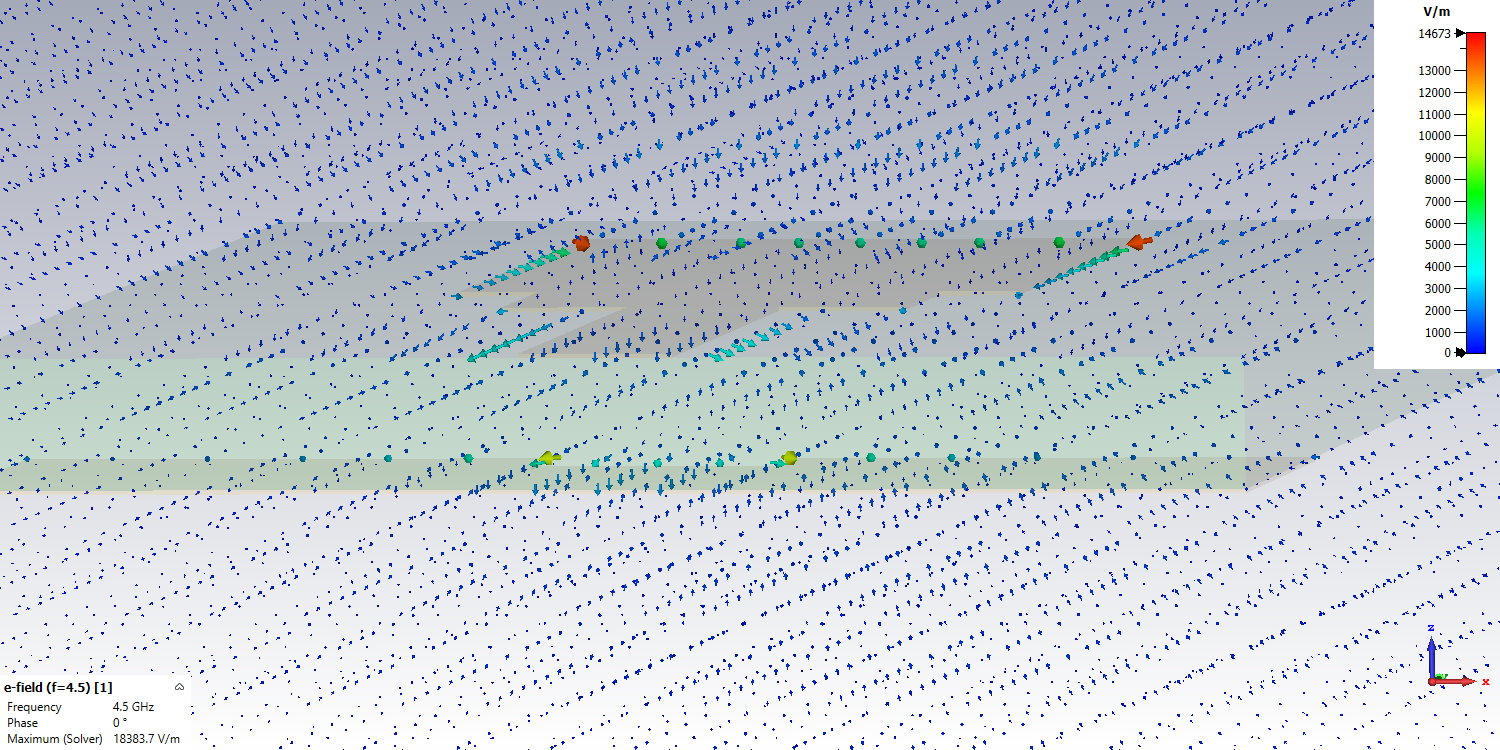
\includegraphics[width=0.3\textwidth]{Images/elec-field-4.5GHz.png}
    	\hfill
		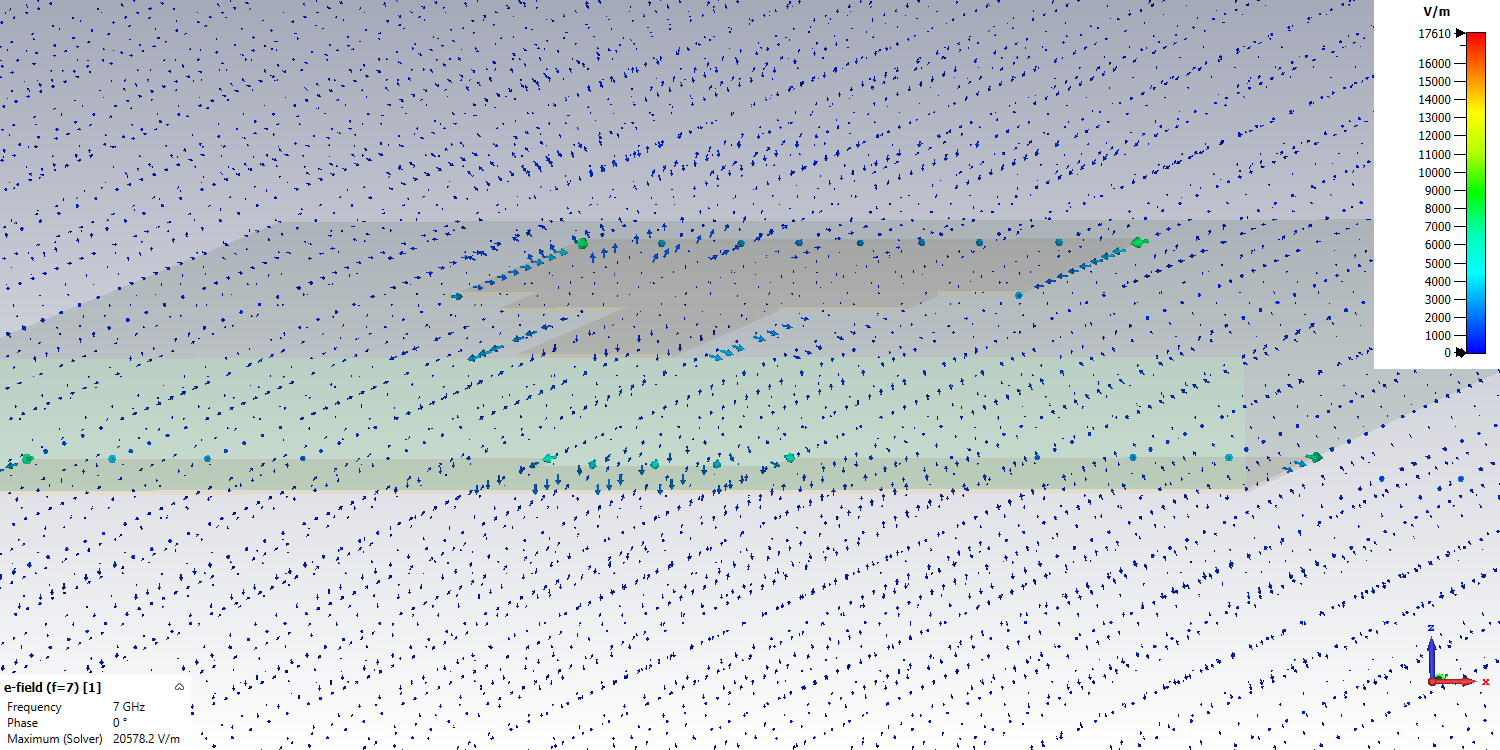
\includegraphics[width=0.3\textwidth]{Images/elec-field-7GHz.png}
		\hfill
		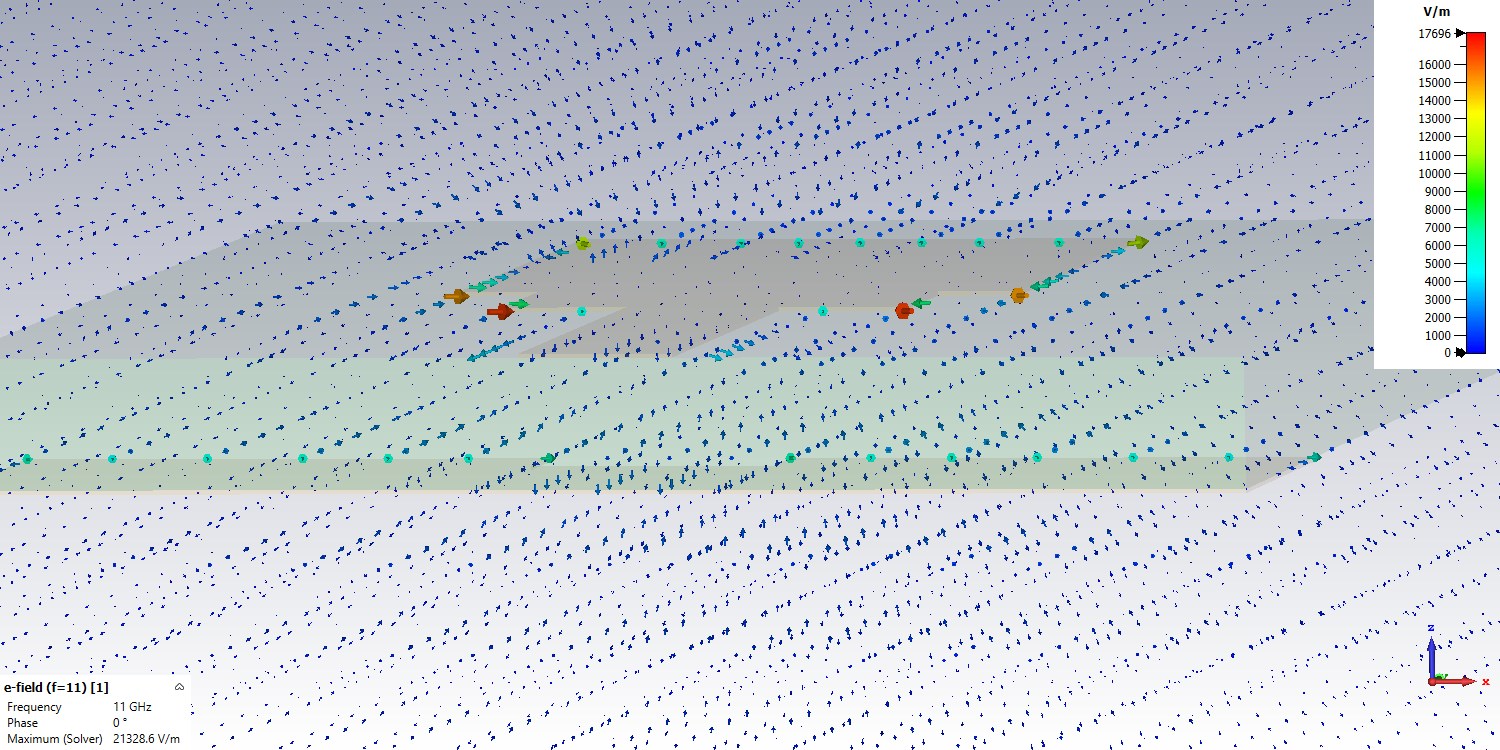
\includegraphics[width=0.3\textwidth]{Images/elec-field-11GHz.png}
	\caption{3D images of the electric field at 4.5GHz, 7GHz, \& 11GHz}\label{fig:electric_field}
\end{figure}

\newpage

The far-field radiation pattern of the antenna at the relevant frequencies (4.5GHz, 7.5GHz, and 11GHz) displays that the resulting antenna does not have a very similar radiation pattern to that of a monopole antenna, it is not as directional as a traditional monopole, the pattern is somewhat similar to a torus shape but not much. At the resonant frequency of 11GHz the torus shape is particularly prominent.
\linebreak

\begin{figure}[ht!]
\centering

		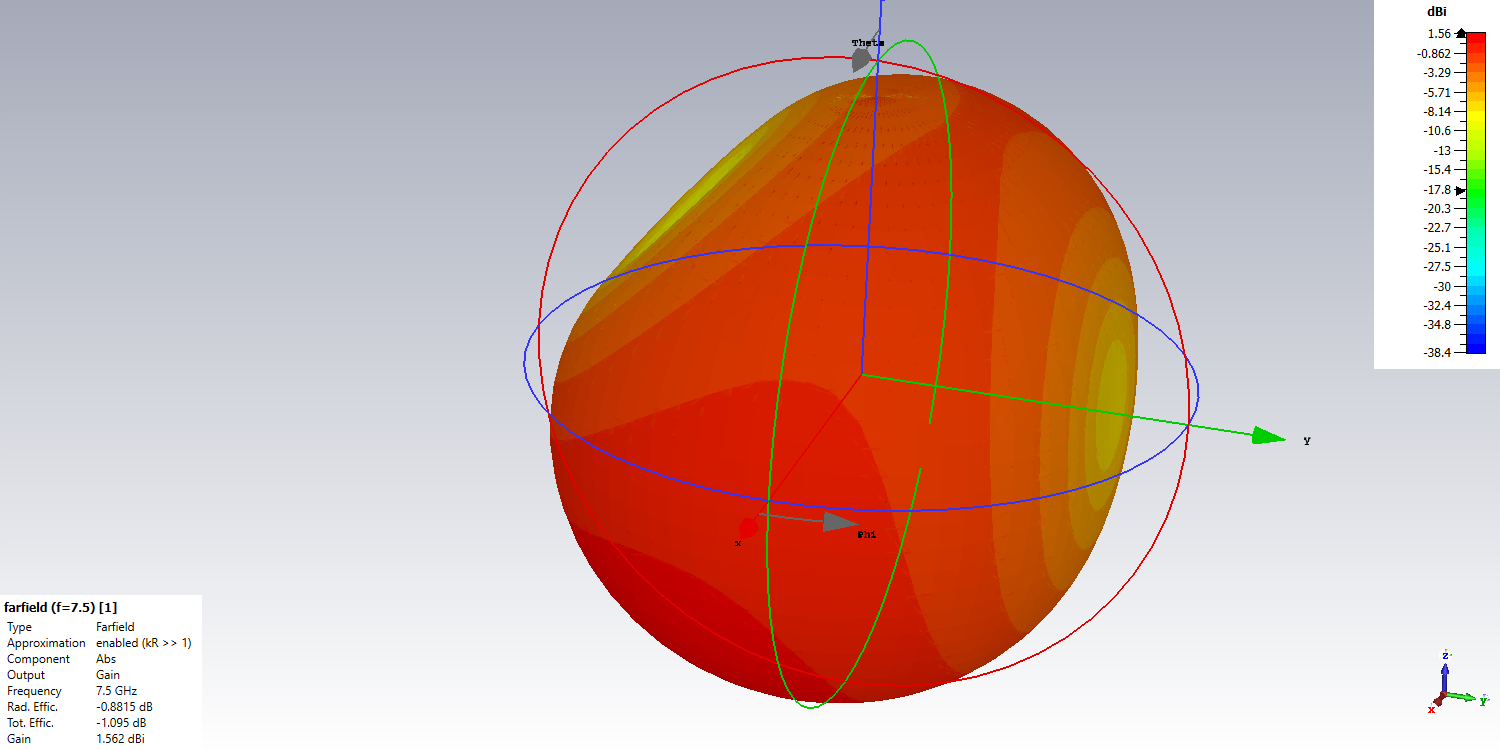
\includegraphics[width=0.3\textwidth]{Images/far-field-4.5GHz.png}
    	\hfill
		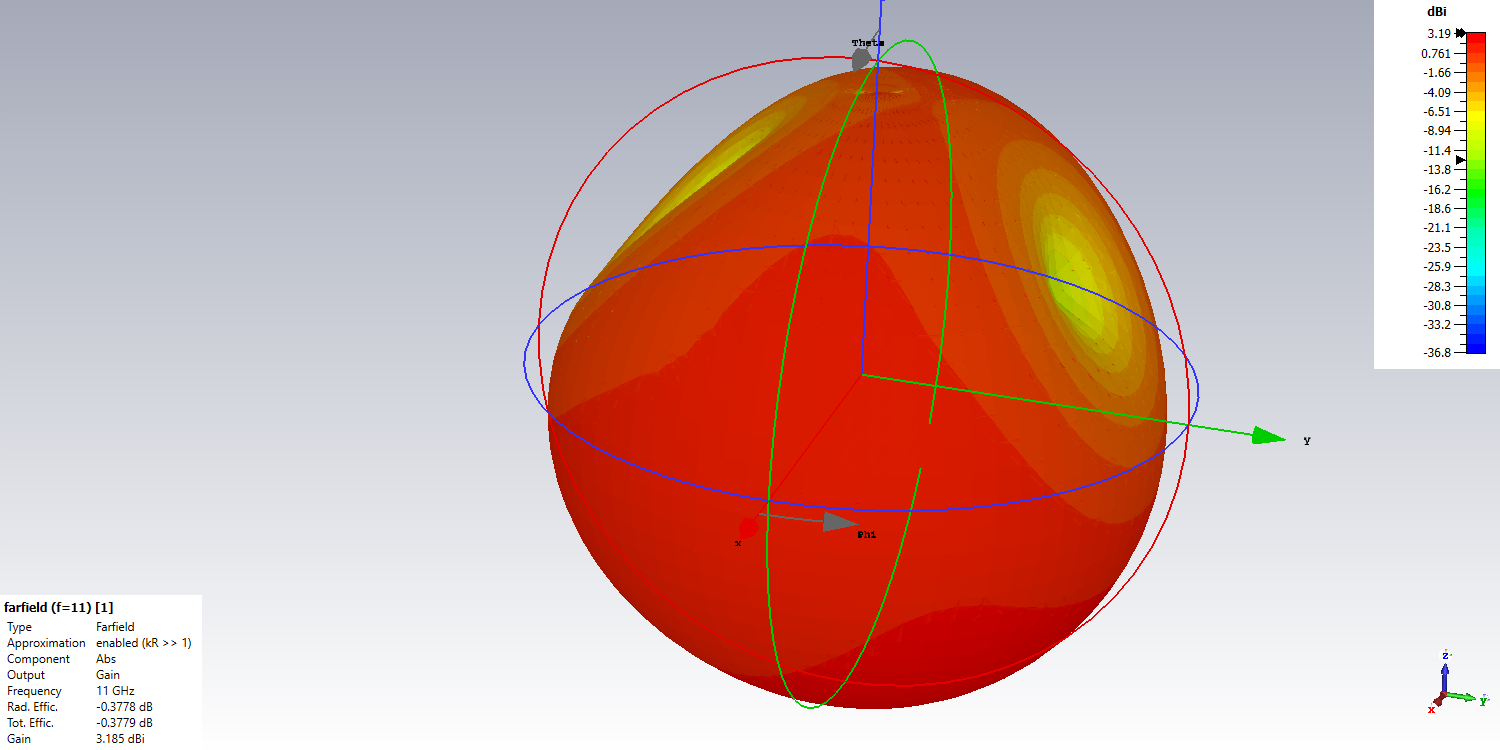
\includegraphics[width=0.3\textwidth]{Images/far-field-7.5GHz.png}
		\hfill
		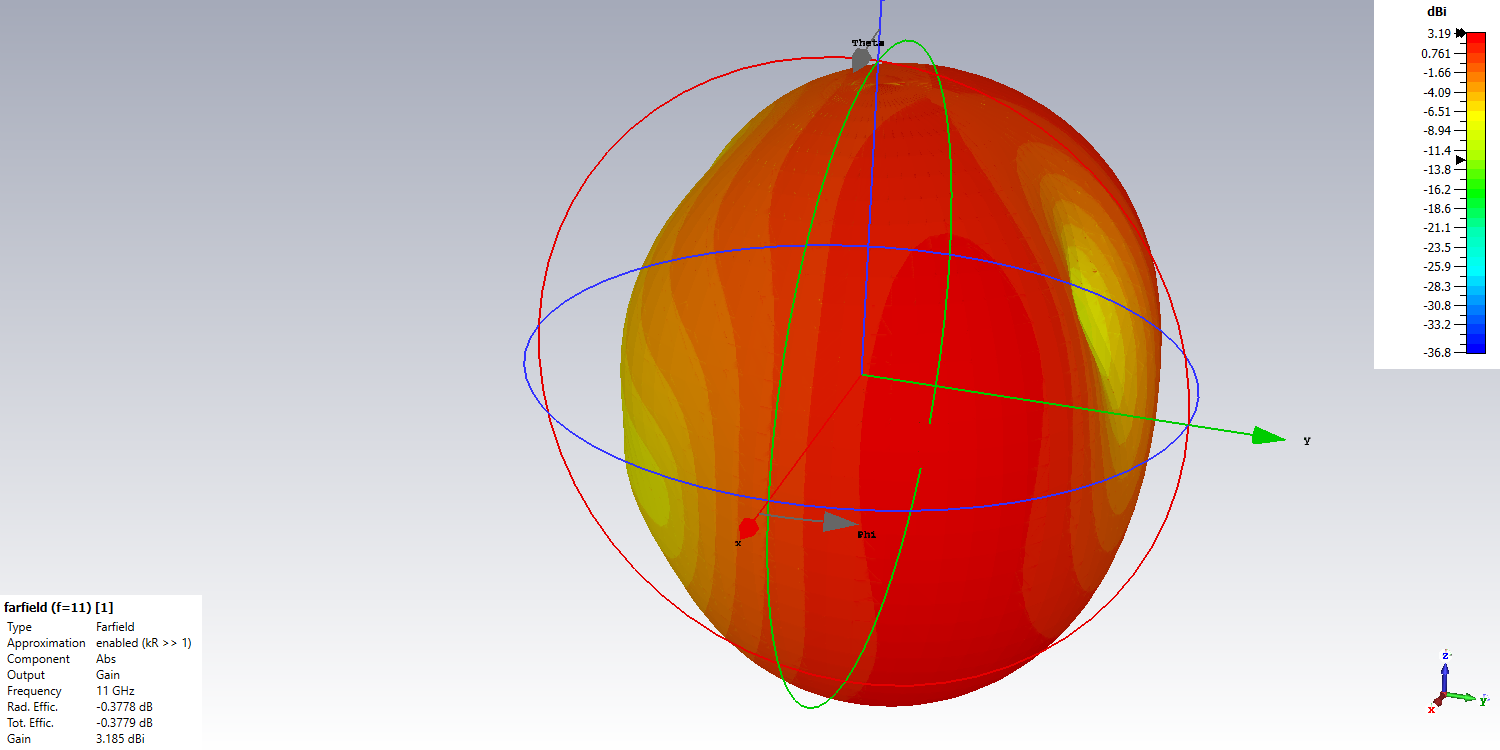
\includegraphics[width=0.3\textwidth]{Images/far-field-11GHz.png}
	\caption{The far-field radiation of the antenna at 4.5GHz, 7.5GHz, \& 11GHz}\label{fig:far-field}
\end{figure}


\newpage
\setstretch{1}  % Reduce bibliography line spacing
\bibliographystyle{IEEEtran}
\bibliography{references.bib}
\end{document}
